\documentclass{scrreprt}
\usepackage{listings}
\usepackage{underscore}
\usepackage{graphicx}
\usepackage[bookmarks=true]{hyperref}
\usepackage[utf8]{inputenc}
\usepackage[english]{babel}
\usepackage{float}
\usepackage{enumitem}
\setlist[itemize]{topsep=4pt, itemsep=4pt, parsep=0pt, partopsep=0pt}
\usepackage{pdflscape}
\usepackage{array}
\usepackage{tabularray}

\UseTblrLibrary{booktabs}
\DefTblrTemplate{firsthead,middlehead,lasthead}{default}{}

\DefTblrTemplate{firstfoot}{default}{
  \UseTblrTemplate{caption}{default}
}

\DefTblrTemplate{middlefoot}{default}{
  \UseTblrTemplate{capcont}{default}
}

\DefTblrTemplate{lastfoot}{default}{
  \UseTblrTemplate{caption}{default}
}

\usepackage[
    a4paper,
    left=2cm,
    right=2cm,
    top=3cm,
    bottom=3cm
]{geometry}


\hypersetup{
    bookmarks=false,    % show bookmarks bar?
    pdftitle={Software Requirement Specification},    % title
    pdfauthor={Vo An Khoi},                     % author
    pdfsubject={SRS for Community Social Network LKForum},
    pdfkeywords={Website, SRS, Social Media},
    colorlinks=true,       % false: boxed links; true: colored links
    linkcolor=blue,       % color of internal links
    citecolor=black,       % color of links to bibliography
    filecolor=black,        % color of file links
    urlcolor=purple,        % color of external links
    linktoc=page            % only page is linked
}%
\def\myversion{1.0 }
\date{}
%\title{%

%}
\usepackage{hyperref}
\begin{document}

\begin{flushright}
    \rule{16cm}{5pt}\vskip1cm
    \begin{bfseries}
        \Huge{SOFTWARE REQUIREMENT \\ SPECIFICATION}\\
        \vspace{1.5cm}
        for\\
        \vspace{1.5cm}
        LKFORUM WEBSITE\\
        \vspace{1.5cm}
        \LARGE{Version \myversion}\\
        \vspace{1.5cm}
        Prepared by : Quach Gia Kiet\\
        Vo An Khoi\\
        \vspace{1.5cm}
        Submitted to : Nguyen Trinh Đong \\Lecturer\\
        \vspace{1.5cm}
        \today\\
    \end{bfseries}
\end{flushright}

\tableofcontents

\chapter{Introduction}

\section{Purpose}
This SRS describes the functional and nonfunctional requirements for software release 1.0 of the Community Social Network Website (LKForum). This document is intended to be used by the members of the project team who will implement and verify the correct functioning of the system. Unless otherwise noted, all requirements specified here are committed for release 1.0

\section{Intended Audience and Reading Suggestions}
This SRS is for developers, project managers, users and testers. Further the discussion will provide all the internal, external, functional and also non-functional informations about "LKFORUM WEBSITE".

\section{Project Scope}
This SRS describes the functional and nonfunctional requirements for software release 1.0 of the Community Social Network Website (LKForum). This document is intended to be used by the members of the project team who will implement and verify the correct functioning of the system. Unless otherwise noted, all requirements specified here are committed for release 1.0

\section{References}

\chapter{Overall Description}

\section{Product Perspective}
Community Social Network LKForum is a new website that provides a comprehensive, modern solution for building and managing online communities. The context diagram in Figure 1 illustrates the external entities and system interfaces for release 1.0. The system is expected to evolve over several releases, ultimately connecting to third-party social media APIs for authentication (Google, Facebook) and expanding to include advanced content monetization tools and mobile-native applications.

\begin{figure}[H]
    \centering
    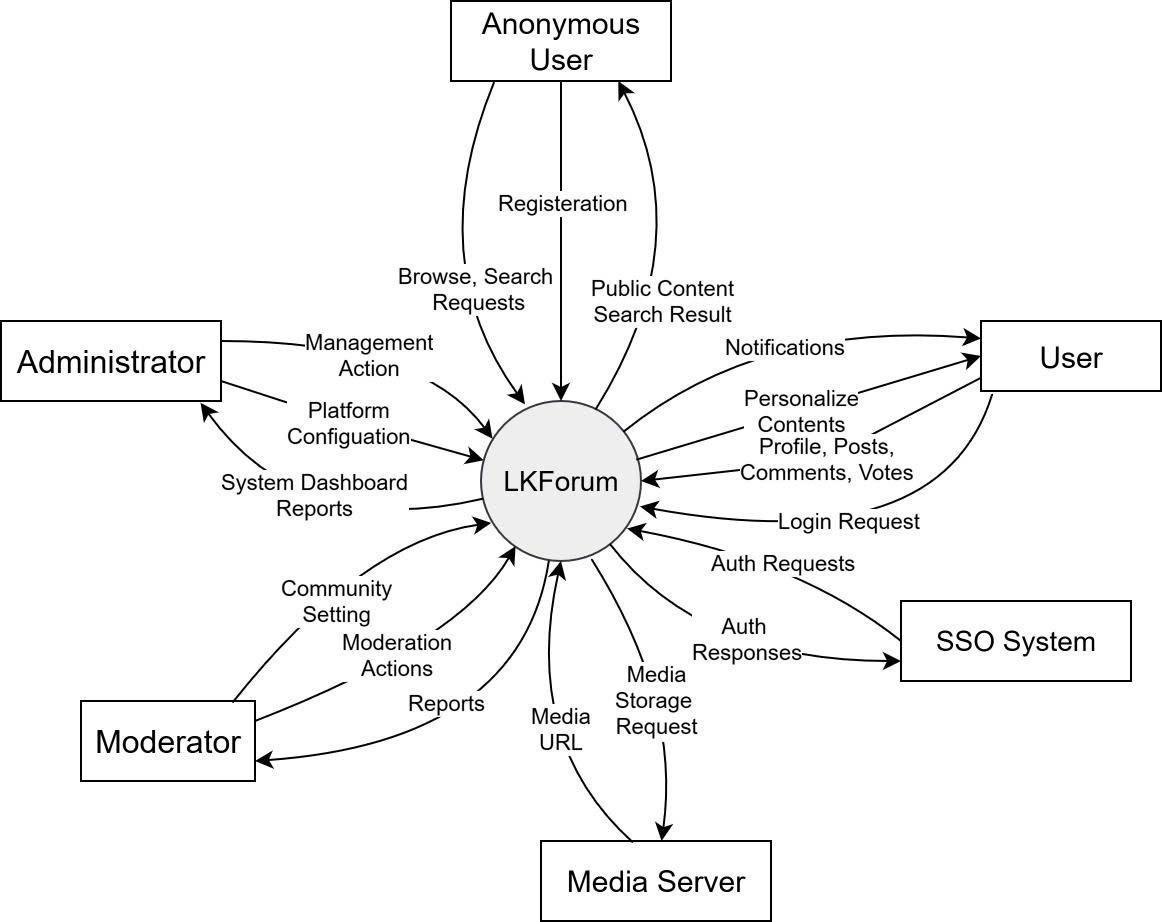
\includegraphics[width=0.8\textwidth]{./diagrams/Context Diagram.jpg}
    \caption{Context diagram for release 1.0 of LKForum}
    \label{fig:context_diagram}
\end{figure}

\section{Operating Environment}

\begin{itemize}[leftmargin=2cm]
    \item[\textbf{OE-1:}] LKForum must operate correctly on modern web browsers including: Google Chrome (latest version), Mozilla Firefox (latest version), Apple Safari (latest version), and Microsoft Edge (latest version).

    \item[\textbf{OE-2:}] Users can access LKForum via the Internet from desktop computers, laptops, and tablets. The interface must have responsive design to be compatible with various screen sizes.
\end{itemize}

\section{Design and Implementation Constraints}

\begin{itemize}[leftmargin=2cm]
    \item[\textbf{CO-1:}] The user interface (front-end) source code must be developed using the Svelte framework.

    \item[\textbf{CO-2:}] The system must use a standard MongoDB NoSQL database with a back-end developed using the Go framework.

    \item[\textbf{CO-3:}] All HTML code must adhere to the HTML 5.0 standard.
\end{itemize}

\section{Assumptions and Dependencies}

\begin{itemize}[leftmargin=2cm]
    \item[\textbf{AS-1:}] It is assumed that users have a stable Internet connection to access and use the platform's features.

    \item[\textbf{DE-1:}] The social media login feature (Google, Facebook) depends on the APIs and policies of these third-party service providers. Any changes on their part may affect the operation of this feature.
\end{itemize}

\chapter{System Features}

The LKForum website is being built using the Go programming language for the back-end, Svelte with Vite for the front-end, MongoDB for primary data storage, and Redis for caching and session management.
\newline
Back-End -- Go with the Gin web framework.
\newline
Front-End -- Svelte with Vite.
\newline
Database -- MongoDB.
\newline
Cache and Session Store -- Redis.

\section{Use Case Description}

\subsection{UC-01 - Sign Up}
\begin{table}[H]
\centering
\begin{tblr}{
    width=\textwidth,
    hlines,
    vlines,
    rows = {valign=m},
    colspec = {Q[l,3cm] Q[l,11cm]}
}
\textbf{Name} & Sign Up \\
\textbf{Description} & This use case describes how a new user creates an account and verifies the email address using OTP. \\
\textbf{Actor} & User \\
\textbf{Trigger} & When the user clicks the ``Sign Up'' button. \\
\textbf{Pre-condition} & The user is not logged in to the system. \newline The user is on the sign up page. \\
\textbf{Post-condition} & The user account is created and verified. \newline The user is authenticated and can access the system. \\
\end{tblr}
\caption{Use Case Specification - Sign Up}
\end{table}

\begin{figure}[H]
    \centering
    
\includegraphics[width=0.8\textwidth]{./diagrams/activity_diagrams/UC_01_Sign_Up.png}
    \caption{Activity Diagram for UC-01}
    \label{fig:ad_uc01}
\end{figure}

\begin{longtblr}[
    caption = {Business Rules for UC-01 - Sign Up},
    label = {tab:uc01_business_rules}
]{
    width=\textwidth,
    hlines,
    vlines,
    rowhead = 1,
    rows = {valign=m, cmd=\nopagebreak},
    row{1} = {font=\bfseries, halign=c},
    colspec = {
        Q[c,1.5cm]
        Q[c,1.5cm]
        Q[l,11cm]
    }
}
\textbf{Activity} & \textbf{BR Code} & \textbf{Description} \\

(4) & BR1 &
\textbf{Validate Email Format:}
\begin{itemize}
    \item The system checks that \textbf{email} is present and valid.
    \item If the \textbf{email} is missing or invalid, the system returns a bad-request error.
\end{itemize} \\

(5--7) & BR2 &
\textbf{Create and Send Verification OTP:}
\begin{itemize}
    \item The system checks whether the \textbf{email} already exists in the user repository.
    \item If the \textbf{email} already exists, the system returns an email-exists error.
    \item Otherwise, the system deletes any existing verification record for the same \textbf{email}.
    \item The system generates a 6-digit \textbf{OTP}, a \textbf{nonce}, and an expiry timestamp using \textbf{\textit{generateOTP()}} and related helpers.
    \item The system stores a new email-verification record with \textbf{IsVerified = false}.
    \item If an email sender is configured, the system sends the \textbf{OTP} by email asynchronously.
\end{itemize} \\

(10--11) & BR3 &
\textbf{Verify OTP and Issue Token:}
\begin{itemize}
    \item The system checks that \textbf{email} and \textbf{otp} are present.
    \item If no verification record exists, the system returns an invalid \textbf{OTP} error.
    \item If the verification record is already marked verified, the system returns an email-already-verified error.
    \item If the \textbf{OTP} does not match or has expired, the system returns an invalid or expired \textbf{OTP} error.
    \item Otherwise, the system marks the verification record as verified.
    \item After successful \textbf{OTP} verification, the system generates a verification token from the verified \textbf{email} and \textbf{nonce}.
    \item The token is returned to the client and is required to complete registration.
\end{itemize} \\

(14) & BR4 &
\textbf{Validate Registration Fields:}
\begin{itemize}
    \item The system checks that \textbf{username} is between 3 and 20 characters.
    \item The system checks that \textbf{password} is at least 8 characters long.
    \item The system checks that the \textbf{password} is strong enough, including uppercase, lowercase, number, and special character, using \textbf{\textit{isStrongPassword()}}.
    \item If any validation fails, the system returns the corresponding error message.
\end{itemize} \\

(15--18) & BR5 &
\textbf{Create Account and Complete Login:}
\begin{itemize}
    \item The system hashes the \textbf{password} with \textbf{\textit{GenerateFromPassword()}} before storing it.
    \item The system checks that the \textbf{username} is still available before creating the account.
    \item The system checks again that the \textbf{email} is still not registered to prevent race conditions.
    \item The system creates the new local user with default settings and \textbf{IsVerified = true}.
    \item The system initializes the user role content and activity stats.
    \item The system deletes the email verification record after successful account creation.
    \item The system invalidates the \textbf{username} cache.
    \item The system generates access and refresh tokens using \textbf{\textit{GenerateToken()}} and returns the auth response.
\end{itemize} \\
\end{longtblr}





\subsection{UC-02 - Sign In}
\begin{table}[H]
\centering
\begin{tblr}{
    width=\textwidth,
    hlines,
    vlines,
    rows = {valign=m},
    colspec = {Q[l,3cm] Q[l,11cm]}
}
\textbf{Name} & Sign In \\
\textbf{Description} & This use case describes how a registered user logs into the system using local credentials or Google OAuth. \\
\textbf{Actor} & User \\
\textbf{Trigger} & When the user clicks the ``Sign In'' button. \\
\textbf{Pre-condition} & The user is not logged in to the system. \newline The user is on the sign in page. \\
\textbf{Post-condition} & The user is authenticated. \newline The user is redirected to the appropriate page. \\
\end{tblr}
\caption{Use Case Specification - Sign In}
\end{table}
\begin{figure}[H]
    \centering
    
\includegraphics[width=0.8\textwidth]{./diagrams/activity_diagrams/UC_02_Local_Sign_In.png}
    \caption{Activity Diagram for UC-02 Local Sign In}
    \label{fig:ad_uc02_local}
\end{figure}
\begin{figure}[H]
    \centering
    
\includegraphics[width=0.8\textwidth]{./diagrams/activity_diagrams/UC_02_Google_Sign_In.png}
    \caption{Activity Diagram for UC-02 Google Sign In}
    \label{fig:ad_uc02_google}
\end{figure}

\subsection{UC-03 - Forgot Password}
\begin{table}[H]
\centering
\begin{tblr}{
    width=\textwidth,
    hlines,
    vlines,
    rows = {valign=m},
    colspec = {Q[l,3cm] Q[l,11cm]}
}
\textbf{Name} & Forgot Password \\
\textbf{Description} & This use case describes how a user resets a forgotten password through email verification and OTP. \\
\textbf{Actor} & User \\
\textbf{Trigger} & When the user clicks the ``Forgot Password'' link. \\
\textbf{Pre-condition} & The user has an existing account and can access the registered email address. \newline The user is not logged in to the system. \\
\textbf{Post-condition} & The user password is reset successfully. \newline The user can sign in again with the new password. \\
\end{tblr}
\caption{Use Case Specification - Forgot Password}
\end{table}


\begin{figure}[H]
    \centering
    
\includegraphics[width=0.8\textwidth]{./diagrams/activity_diagrams/UC_03_Forgot_Password.png}
    \caption{Activity Diagram for UC-03}
    \label{fig:ad_uc03}
\end{figure}

\begin{longtblr}[
    caption = {Business Rules for UC-03 - Forgot Password},
    label = {tab:uc03_business_rules}
]{
    width=\textwidth,
    hlines,
    vlines,
    rowhead = 1,
    rows = {valign=m, cmd=\nopagebreak},
    row{1} = {font=\bfseries, halign=c},
    colspec = {
        Q[c,1.5cm]
        Q[c,1.5cm]
        Q[l,11cm]
    }
}
\textbf{Activity} & \textbf{BR Code} & \textbf{Description} \\

(4) & BR1 &
\textbf{Validate Reset Request:}
\begin{itemize}
    \item The system checks that \textbf{email} is present and valid.
    \item The system looks up the account by \textbf{email} using \textbf{\textit{GetByEmail()}}.
    \item If the account does not exist, the system returns an email-not-registered error.
    \item If the account exists but the \textbf{provider} is not local, the system returns a login-method-mismatch error.
\end{itemize} \\

(5--7) & BR2 &
\textbf{Create Password Reset Request:}
\begin{itemize}
    \item The system deletes any existing reset record for the same \textbf{email} so the user can request a new OTP.
    \item The system generates a 6-digit \textbf{OTP}, a \textbf{nonce}, and an expiry timestamp using \textbf{\textit{generateOTP()}} and \textbf{\textit{generateNonce()}}.
    \item The system stores a new password-reset record with \textbf{IsVerified = false}.
    \item If an email sender is configured, the system sends the reset OTP asynchronously using \textbf{\textit{SendPasswordResetEmail()}}.
\end{itemize} \\

(10--11) & BR3 &
\textbf{Verify Reset OTP and Issue Token:}
\begin{itemize}
    \item The system checks that \textbf{email} and \textbf{otp} are present.
    \item If no reset record exists, the system returns an invalid \textbf{OTP} error.
    \item If the reset record is already verified, the system returns an email-already-verified error.
    \item If the \textbf{OTP} does not match or has expired, the system returns an invalid or expired \textbf{OTP} error.
    \item Otherwise, the system marks the reset record as verified.
    \item The system generates a reset token from the verified \textbf{email} and \textbf{nonce} using \textbf{\textit{CreateVerificationToken()}}.
\end{itemize} \\

(14--16) & BR4 &
\textbf{Reset Password:}
\begin{itemize}
    \item The system checks that \textbf{newPassword} is at least 8 characters long.
    \item The system checks that \textbf{newPassword} is strong enough using \textbf{\textit{isStrongPassword()}}.
    \item The system parses the reset token using \textbf{\textit{auth.ParseVerificationToken()}} and verifies the stored \textbf{nonce}.
    \item The system hashes \textbf{newPassword} with \textbf{\textit{GenerateFromPassword()}} and updates the user account.
    \item The system deletes the reset record after a successful password change.
\end{itemize} \\
\end{longtblr}


\subsection{UC-04 - Manage Profile}
\begin{table}[H]
\centering
\begin{tblr}{
    width=\textwidth,
    hlines,
    vlines,
    rows = {valign=m},
    colspec = {Q[l,3cm] Q[l,11cm]}
}
\textbf{Name} & Manage Profile \\
\textbf{Description} & This use case describes how a user updates profile information such as bio, avatar, and cover image. \\
\textbf{Actor} & User \\
\textbf{Trigger} & When the user opens the profile edit page. \\
\textbf{Pre-condition} & The user is logged in to the system. \newline The user has permission to edit the profile. \\
\textbf{Post-condition} & The profile information is updated and stored. \newline The new profile data is visible across the system. \\
\end{tblr}
\caption{Use Case Specification - Manage Profile}
\end{table}


\begin{figure}[H]
    \centering
    
\includegraphics[width=0.8\textwidth]{./diagrams/activity_diagrams/UC_04_Manage_Profile.png}
    \caption{Activity Diagram for UC-04}
    \label{fig:ad_uc04}
\end{figure}

\begin{longtblr}[
    caption = {Business Rules for UC-04 - Manage Profile},
    label = {tab:uc04_business_rules}
]{
    width=\textwidth,
    hlines,
    vlines,
    rowhead = 1,
    rows = {valign=m, cmd=\nopagebreak},
    row{1} = {font=\bfseries, halign=c},
    colspec = {
        Q[c,1.5cm]
        Q[c,1.5cm]
        Q[l,11cm]
    }
}
\textbf{Activity} & \textbf{BR Code} & \textbf{Description} \\

(5) & BR1 &
\textbf{Validate Profile Fields:}
\begin{itemize}
    \item The system checks the submitted profile fields before saving.
    \item \textbf{bio} is limited by DTO validation, \textbf{gender} must match a valid model value, and \textbf{date\_of\_birth} must parse as a valid date.
    \item The system validates \textbf{location} against allowed provinces and ensures \textbf{interests} do not exceed the maximum allowed count.
\end{itemize} \\

(6) & BR2 &
\textbf{Update Profile Data:}
\begin{itemize}
    \item The system loads the current user and updates \textbf{RoleContent.AsUser}.
    \item Empty string values clear the corresponding profile field.
    \item Invalid \textbf{gender}, \textbf{location}, or \textbf{interest} values return an error instead of being saved.
\end{itemize} \\

(7--8) & BR3 &
\textbf{Upload and Save Profile Images:}
\begin{itemize}
    \item When the user uploads an avatar or cover image, the system sends the file to \textbf{\textit{cloudinary.UploadImages()}}.
    \item The system stores the returned image \textbf{URL} and \textbf{PublicID} through \textbf{\textit{UpdateAvatar()}} or \textbf{\textit{UpdateCover()}}.
    \item If an older image exists, the system deletes the old asset asynchronously using \textbf{\textit{cloudinary.Delete()}}.
\end{itemize} \\

(9) & BR4 &
\textbf{Return Updated Profile:}
\begin{itemize}
    \item The system returns the refreshed user profile after saving changes.
\end{itemize} \\
\end{longtblr}


\subsection{UC-05 - Change Settings}
\begin{table}[H]
\centering
\begin{tblr}{
    width=\textwidth,
    hlines,
    vlines,
    rows = {valign=m},
    colspec = {Q[l,3cm] Q[l,11cm]}
}
\textbf{Name} & Change Settings \\
\textbf{Description} & This use case describes how a user changes account preferences such as privacy, notifications, and theme. \\
\textbf{Actor} & User \\
\textbf{Trigger} & When the user opens the settings page. \\
\textbf{Pre-condition} & The user is logged in to the system. \newline The settings page is available to the user. \\
\textbf{Post-condition} & The selected preferences are saved. \newline The account settings are updated for future sessions. \\
\end{tblr}
\caption{Use Case Specification - Change Settings}
\end{table}


\begin{figure}[H]
    \centering
    
\includegraphics[width=0.8\textwidth]{./diagrams/activity_diagrams/UC_05_Change_Settings.png}
    \caption{Activity Diagram for UC-05}
    \label{fig:ad_uc05}
\end{figure}


\begin{longtblr}[
    caption = {Business Rules for UC-05 - Change Settings},
    label = {tab:uc05_business_rules}
]{
    width=\textwidth,
    hlines,
    vlines,
    rowhead = 1,
    rows = {valign=m, cmd=\nopagebreak},
    row{1} = {font=\bfseries, halign=c},
    colspec = {
        Q[c,1.5cm]
        Q[c,1.5cm]
        Q[l,11cm]
    }
}
\textbf{Activity} & \textbf{BR Code} & \textbf{Description} \\

(2--3) & BR1 &
\textbf{Load Current Settings:}
\begin{itemize}
    \item The system loads the user's current \textbf{Settings} from the database using \textbf{\textit{GetSettings()}}.
    \item If the user has no settings record, the system returns default settings through \textbf{\textit{dto.FromSettings()}}.
\end{itemize} \\

(6) & BR2 &
\textbf{Validate Settings Values:}
\begin{itemize}
    \item The system validates \textbf{theme} and \textbf{fontSize} using \textbf{\textit{model.IsValidTheme()}} and \textbf{\textit{model.IsValidFontSize()}}.
    \item The system accepts only values supported by the model enums and returns a bad-request error for invalid input.
\end{itemize} \\

(7--8) & BR3 &
\textbf{Persist Updated Settings:}
\begin{itemize}
    \item The system updates \textbf{Appearance}, \textbf{Notifications}, \textbf{Privacy}, and \textbf{Content} fields in \textbf{user.Settings}.
    \item The system saves the updated user record with \textbf{\textit{userRepo.Update()}}.
    \item The system returns the updated settings after persistence.
\end{itemize} \\
\end{longtblr}


\subsection{UC-06 - View Activity History}
\begin{table}[H]
\centering
\begin{tblr}{
    width=\textwidth,
    hlines,
    vlines,
    rows = {valign=m},
    colspec = {Q[l,3cm] Q[l,11cm]}
}
\textbf{Name} & View Activity History \\
\textbf{Description} & This use case describes how a user reviews past posts, comments, and interactions. \\
\textbf{Actor} & User \\
\textbf{Trigger} & When the user opens the activity history page. \\
\textbf{Pre-condition} & The user is logged in to the system. \newline The user has activity records in the system. \\
\textbf{Post-condition} & The activity history is displayed to the user. \newline The user can review prior activity. \\
\end{tblr}
\caption{Use Case Specification - View Activity History}
\end{table}


\begin{figure}[H]
    \centering

\includegraphics[width=0.8\textwidth]{./diagrams/activity_diagrams/UC_06_View_Activity_History.png}
    \caption{Activity Diagram for UC-06}
    \label{fig:ad_uc06}
\end{figure}

\begin{longtblr}[
    caption = {Business Rules for UC-06 - View Activity History},
    label = {tab:uc06_business_rules}
]{
    width=\textwidth,
    hlines,
    vlines,
    rowhead = 1,
    rows = {valign=m, cmd=\nopagebreak},
    row{1} = {font=\bfseries, halign=c},
    colspec = {
        Q[c,1.5cm]
        Q[c,1.5cm]
        Q[l,11cm]
    }
}
\textbf{Activity} & \textbf{BR Code} & \textbf{Description} \\

(3--5) & BR1 &
\textbf{Validate Ownership and Fetch History:}
\begin{itemize}
    \item The system checks that the requester is authenticated and that \textbf{userID} matches the current user for the history request.
    \item The system fetches paginated post history using \textbf{\textit{GetPostHistoryByUserID()}}.
    \item If no records are found, the system returns an empty result with pagination data.
\end{itemize} \\

(7) & BR2 &
\textbf{Return Selected History Record:}
\begin{itemize}
    \item The system returns a single history item only when the requester owns the record.
    \item The system rejects access if \textbf{requesterID} does not match the stored \textbf{UserID}.
\end{itemize} \\
\end{longtblr}


\subsection{UC-07 - Follow / Unfollow User}
\begin{table}[H]
\centering
\begin{tblr}{
    width=\textwidth,
    hlines,
    vlines,
    rows = {valign=m},
    colspec = {Q[l,3cm] Q[l,11cm]}
}
\textbf{Name} & Follow / Unfollow User \\
\textbf{Description} & This use case describes how a user subscribes to or unsubscribes from another user's activity feed. \\
\textbf{Actor} & User \\
\textbf{Trigger} & When the user clicks the follow or unfollow action on another profile. \\
\textbf{Pre-condition} & The user is logged in to the system. \newline The target profile is available for follow actions. \\
\textbf{Post-condition} & The follow relationship is created or removed. \newline The user's feed and follower lists are updated. \\
\end{tblr}
\caption{Use Case Specification - Follow / Unfollow User}
\end{table}


\begin{figure}[H]
    \centering
    
\includegraphics[width=0.8\textwidth]{./diagrams/activity_diagrams/UC_07_Follow_Unfollow_User.png}
    \caption{Activity Diagram for UC-07}
    \label{fig:ad_uc07}
\end{figure}

\begin{longtblr}[
    caption = {Business Rules for UC-07 - Follow / Unfollow User},
    label = {tab:uc07_business_rules}
]{
    width=\textwidth,
    hlines,
    vlines,
    rowhead = 1,
    rows = {valign=m, cmd=\nopagebreak},
    row{1} = {font=\bfseries, halign=c},
    colspec = {
        Q[c,1.5cm]
        Q[c,1.5cm]
        Q[l,11cm]
    }
}
\textbf{Activity} & \textbf{BR Code} & \textbf{Description} \\

(3--6) & BR1 &
\textbf{Backend Rule Status:}
\begin{itemize}
    \item No follow or unfollow route, controller, or service is present in the backend code.
    \item The repository currently has no server-side business rules to define for this use case.
    \item This use case remains documented-only until a backend implementation is added.
\end{itemize} \\
\end{longtblr}


\subsection{UC-08 - Browse Content}
\begin{table}[H]
\centering
\begin{tblr}{
    width=\textwidth,
    hlines,
    vlines,
    rows = {valign=m},
    colspec = {Q[l,3cm] Q[l,11cm]}
}
\textbf{Name} & Browse Content \\
\textbf{Description} & This use case describes how a visitor or user explores communities and public posts. \\
\textbf{Actor} & Guest User / User \\
\textbf{Trigger} & When the user opens the forum homepage or a community page. \\
\textbf{Pre-condition} & The browsing page is accessible. \newline The user may be logged in or not logged in. \\
\textbf{Post-condition} & Public posts and community content are shown. \newline The user can continue browsing or open a post. \\
\end{tblr}
\caption{Use Case Specification - Browse Content}
\end{table}


\begin{figure}[H]
    \centering
    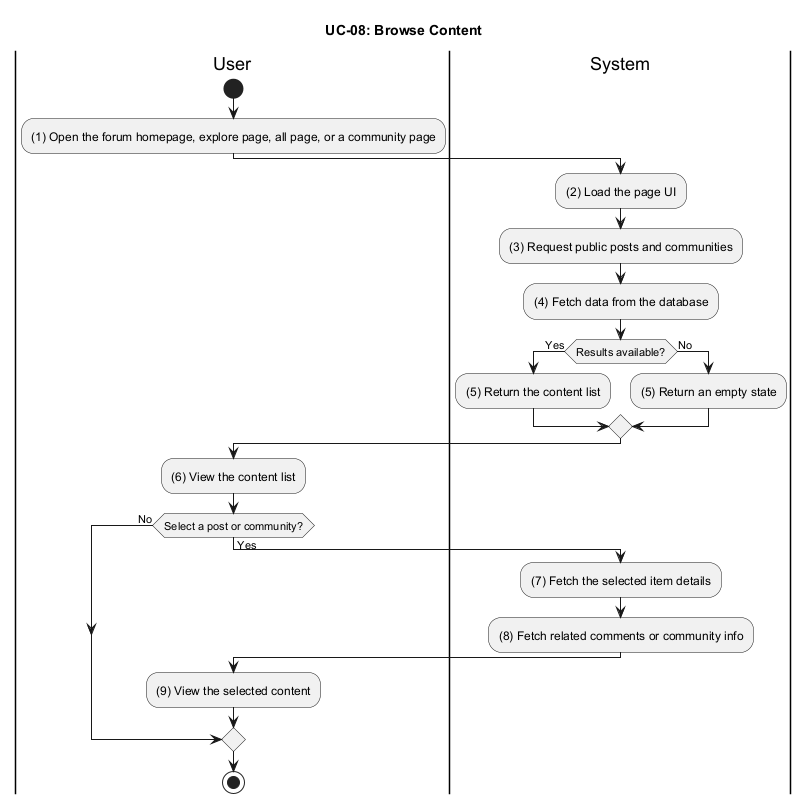
\includegraphics[width=0.8\textwidth]{./diagrams/activity_diagrams/UC_08_Browse_Content.png}
    \caption{Activity Diagram for UC-08}
    \label{fig:ad_uc08}
\end{figure}

\begin{longtblr}[
    caption = {Business Rules for UC-08 - Browse Content},
    label = {tab:uc08_business_rules}
]{
    width=\textwidth,
    hlines,
    vlines,
    rowhead = 1,
    rows = {valign=m, cmd=\nopagebreak},
    row{1} = {font=\bfseries, halign=c},
    colspec = {
        Q[c,1.5cm]
        Q[c,1.5cm]
        Q[l,11cm]
    }
}
\textbf{Activity} & \textbf{BR Code} & \textbf{Description} \\

(2--5) & BR1 &
\textbf{Load Public Content:}
\begin{itemize}
    \item The system loads the page UI and requests public posts and communities.
    \item The system fetches content from the database using \textbf{\textit{GetPosts()}} and community lookup functions.
    \item If no results exist, the system returns an empty state instead of an error.
\end{itemize} \\

(7--9) & BR2 &
\textbf{Open Selected Content:}
\begin{itemize}
    \item If the user selects a post, the system loads the post details using \textbf{\textit{GetPostByID()}}.
    \item If the user selects a community, the system loads the community details using \textbf{\textit{GetCommunityByID()}} or \textbf{\textit{GetCommunityByName()}}.
    \item The system also returns related comments or community information for the selected item.
\end{itemize} \\
\end{longtblr}


\subsection{UC-09 - Search Content}
\begin{table}[H]
\centering
\begin{tblr}{
    width=\textwidth,
    hlines,
    vlines,
    rows = {valign=m},
    colspec = {Q[l,3cm] Q[l,11cm]}
}
\textbf{Name} & Search Content \\
\textbf{Description} & This use case describes how a user searches for posts, users, or communities by keyword. \\
\textbf{Actor} & User \\
\textbf{Trigger} & When the user enters a search term and submits the search. \\
\textbf{Pre-condition} & The search page is available. \newline The system has searchable content. \\
\textbf{Post-condition} & Matching results are returned to the user. \newline The user can open a result or refine the search. \\
\end{tblr}
\caption{Use Case Specification - Search Content}
\end{table}


\begin{figure}[H]
    \centering
    
\includegraphics[width=0.8\textwidth]{./diagrams/activity_diagrams/UC_09_Search_Content.png}
    \caption{Activity Diagram for UC-09}
    \label{fig:ad_uc09}
\end{figure}

\begin{longtblr}[
    caption = {Business Rules for UC-09 - Search Content},
    label = {tab:uc09_business_rules}
]{
    width=\textwidth,
    hlines,
    vlines,
    rowhead = 1,
    rows = {valign=m, cmd=\nopagebreak},
    row{1} = {font=\bfseries, halign=c},
    colspec = {
        Q[c,1.5cm]
        Q[c,1.5cm]
        Q[l,11cm]
    }
}
\textbf{Activity} & \textbf{BR Code} & \textbf{Description} \\

(4--6) & BR1 &
\textbf{Normalize and Search in Parallel:}
\begin{itemize}
    \item The system normalizes the query before searching.
    \item The system searches posts, users, and communities in parallel using \textbf{\textit{GetPosts()}}, \textbf{\textit{GetUsers()}}, and \textbf{\textit{GetCommunitiesFilter()}}.
    \item If no results are found, the system returns an empty result set.
\end{itemize} \\

(8) & BR2 &
\textbf{Open Search Result:}
\begin{itemize}
    \item If the user opens a result, the system loads the selected post, user profile, or community page.
    \item The system uses the corresponding detail lookup function based on the result type.
\end{itemize} \\
\end{longtblr}


\subsection{UC-10 - Create Post}
\begin{table}[H]
\centering
\begin{tblr}{
    width=\textwidth,
    hlines,
    vlines,
    rows = {valign=m},
    colspec = {Q[l,3cm] Q[l,11cm]}
}
\textbf{Name} & Create Post \\
\textbf{Description} & This use case describes how a member creates and submits a new post in a community. \\
\textbf{Actor} & User \\
\textbf{Trigger} & When the user clicks the ``Create Post'' action. \\
\textbf{Pre-condition} & The user is logged in to the system. \newline The user is a member of the selected community. \\
\textbf{Post-condition} & The post is stored successfully. \newline The post appears in the community or enters moderation if required. \\
\end{tblr}
\caption{Use Case Specification - Create Post}
\end{table}


\begin{figure}[H]
    \centering
    
\includegraphics[width=0.8\textwidth]{./diagrams/activity_diagrams/UC_10_Create_Post.png}
    \caption{Activity Diagram for UC-10}
    \label{fig:ad_uc10}
\end{figure}


\begin{longtblr}[
    caption = {Business Rules for UC-10 - Create Post},
    label = {tab:uc10_business_rules}
]{
    width=\textwidth,
    hlines,
    vlines,
    rowhead = 1,
    rows = {valign=m, cmd=\nopagebreak},
    row{1} = {font=\bfseries, halign=c},
    colspec = {
        Q[c,1.5cm]
        Q[c,1.5cm]
        Q[l,11cm]
    }
}
\textbf{Activity} & \textbf{BR Code} & \textbf{Description} \\

(5) & BR1 &
\textbf{Validate Author and Community:}
\begin{itemize}
    \item The system checks that the user is authenticated and is a member of the selected community.
    \item The system rejects the request if the community is banned or the user is banned from the community.
\end{itemize} \\

(6) & BR2 &
\textbf{Create the Post Record:}
\begin{itemize}
    \item The system creates the post with the submitted \textbf{title}, \textbf{content}, \textbf{tags}, and \textbf{type}.
    \item The system sets the initial moderation state based on community approval rules and author role.
    \item The system auto-upvotes the post for the creator using \textbf{\textit{VoteOnTargetByAuthor()}}.
\end{itemize} \\

(7--8) & BR3 &
\textbf{Handle Media and Poll Data:}
\begin{itemize}
    \item If images or videos are attached, the system uploads them using \textbf{\textit{UploadImages()}} or \textbf{\textit{UploadVideos()}}.
    \item If a poll is included, the system stores poll options and poll settings in the post content.
\end{itemize} \\

(9) & BR4 &
\textbf{Return Created Post:}
\begin{itemize}
    \item The system returns the created post after persistence and moderation setup are complete.
\end{itemize} \\
\end{longtblr}


\subsection{UC-11 - Edit Post}
\begin{table}[H]
\centering
\begin{tblr}{
    width=\textwidth,
    hlines,
    vlines,
    rows = {valign=m},
    colspec = {Q[l,3cm] Q[l,11cm]}
}
\textbf{Name} & Edit Post \\
\textbf{Description} & This use case describes how a member modifies an existing post and preserves edit history. \\
\textbf{Actor} & User \\
\textbf{Trigger} & When the user opens an existing post and chooses ``Edit''. \\
\textbf{Pre-condition} & The user is logged in to the system. \newline The user owns the post or has edit permission. \\
\textbf{Post-condition} & The edited post is saved successfully. \newline The edit history is retained. \\
\end{tblr}
\caption{Use Case Specification - Edit Post}
\end{table}


\begin{figure}[H]
    \centering
    
\includegraphics[width=0.8\textwidth]{./diagrams/activity_diagrams/UC_11_Edit_Post.png}
    \caption{Activity Diagram for UC-11}
    \label{fig:ad_uc11}
\end{figure}


\begin{longtblr}[
    caption = {Business Rules for UC-11 - Edit Post},
    label = {tab:uc11_business_rules}
]{
    width=\textwidth,
    hlines,
    vlines,
    rowhead = 1,
    rows = {valign=m, cmd=\nopagebreak},
    row{1} = {font=\bfseries, halign=c},
    colspec = {
        Q[c,1.5cm]
        Q[c,1.5cm]
        Q[l,11cm]
    }
}
\textbf{Activity} & \textbf{BR Code} & \textbf{Description} \\

(2--4) & BR1 &
\textbf{Authorize Editing:}
\begin{itemize}
    \item The system loads the post and verifies that the requester is the author.
    \item If the requester is not the author, the system returns a forbidden error.
\end{itemize} \\

(5--6) & BR2 &
\textbf{Apply Content Changes:}
\begin{itemize}
    \item The system updates \textbf{title}, \textbf{text}, and \textbf{tags} when they are provided.
    \item If no fields change, the system returns the current post without modifying data.
\end{itemize} \\

(7--11) & BR3 &
\textbf{Handle Media Updates:}
\begin{itemize}
    \item If media is removed, the system deletes the old assets using \textbf{\textit{Delete()}}.
    \item If new media is uploaded, the system stores it using \textbf{\textit{UploadImages()}} or \textbf{\textit{UploadVideos()}}.
    \item The system persists the updated media links back to the post record.
\end{itemize} \\

(12) & BR4 &
\textbf{Return Updated Post:}
\begin{itemize}
    \item The system returns the refreshed post after the update is saved.
\end{itemize} \\
\end{longtblr}


\subsection{UC-12 - Delete Post}
\begin{table}[H]
\centering
\begin{tblr}{
    width=\textwidth,
    hlines,
    vlines,
    rows = {valign=m},
    colspec = {Q[l,3cm] Q[l,11cm]}
}
\textbf{Name} & Delete Post \\
\textbf{Description} & This use case describes how a member or moderator removes a post from public view using soft delete. \\
\textbf{Actor} & User / Moderator \\
\textbf{Trigger} & When the user clicks the ``Delete'' action on a post. \\
\textbf{Pre-condition} & The user is logged in to the system. \newline The user has permission to delete the post. \\
\textbf{Post-condition} & The post is marked as deleted. \newline The post is hidden from public view. \\
\end{tblr}
\caption{Use Case Specification - Delete Post}
\end{table}


\begin{figure}[H]
    \centering
    
\includegraphics[width=0.8\textwidth]{./diagrams/activity_diagrams/UC_12_Delete_Post.png}
    \caption{Activity Diagram for UC-12}
    \label{fig:ad_uc12}
\end{figure}


\begin{longtblr}[
    caption = {Business Rules for UC-12 - Delete Post},
    label = {tab:uc12_business_rules}
]{
    width=\textwidth,
    hlines,
    vlines,
    rowhead = 1,
    rows = {valign=m, cmd=\nopagebreak},
    row{1} = {font=\bfseries, halign=c},
    colspec = {
        Q[c,1.5cm]
        Q[c,1.5cm]
        Q[l,11cm]
    }
}
\textbf{Activity} & \textbf{BR Code} & \textbf{Description} \\

(4--5) & BR1 &
\textbf{Verify Delete Permission:}
\begin{itemize}
    \item The system loads the post record and checks whether the requester is the author.
    \item If the requester is not the author, the system checks for admin, creator, or moderator permission.
    \item If no permission exists, the system returns a forbidden error.
\end{itemize} \\

(6--8) & BR2 &
\textbf{Soft Delete the Post:}
\begin{itemize}
    \item The system marks the post as deleted in storage.
    \item If the author deletes their own post, the system decreases the author's post count.
    \item The system returns a delete success response.
\end{itemize} \\
\end{longtblr}


\subsection{UC-13 - Post Comment}
\begin{table}[H]
\centering
\begin{tblr}{
    width=\textwidth,
    hlines,
    vlines,
    rows = {valign=m},
    colspec = {Q[l,3cm] Q[l,11cm]}
}
\textbf{Name} & Post Comment \\
\textbf{Description} & This use case describes how a user adds a direct comment to a post. \\
\textbf{Actor} & User \\
\textbf{Trigger} & When the user submits a comment on a post. \\
\textbf{Pre-condition} & The user is logged in to the system. \newline The target post is visible and commentable. \\
\textbf{Post-condition} & The comment is created and attached to the post. \newline The comment count is updated. \\
\end{tblr}
\caption{Use Case Specification - Post Comment}
\end{table}


\begin{figure}[H]
    \centering
    
\includegraphics[width=0.8\textwidth]{./diagrams/activity_diagrams/UC_13_Post_Comment.png}
    \caption{Activity Diagram for UC-13}
    \label{fig:ad_uc13}
\end{figure}


\begin{longtblr}[
    caption = {Business Rules for UC-13 - Post Comment},
    label = {tab:uc13_business_rules}
]{
    width=\textwidth,
    hlines,
    vlines,
    rowhead = 1,
    rows = {valign=m, cmd=\nopagebreak},
    row{1} = {font=\bfseries, halign=c},
    colspec = {
        Q[c,1.5cm]
        Q[c,1.5cm]
        Q[l,11cm]
    }
}
\textbf{Activity} & \textbf{BR Code} & \textbf{Description} \\

(4) & BR1 &
\textbf{Validate Post and Permissions:}
\begin{itemize}
    \item The system validates authentication and checks that the target post exists.
    \item The system blocks the comment if the user is banned or muted in the post's community.
\end{itemize} \\

(5--7) & BR2 &
\textbf{Create the Comment:}
\begin{itemize}
    \item The system stores the new comment with the current user as author.
    \item The system increments the post comment count and the user's comment count.
    \item The system publishes the comment-created event for follow-up processing.
\end{itemize} \\
\end{longtblr}


\subsection{UC-14 - Reply to Comment}
\begin{table}[H]
\centering
\begin{tblr}{
    width=\textwidth,
    hlines,
    vlines,
    rows = {valign=m},
    colspec = {Q[l,3cm] Q[l,11cm]}
}
\textbf{Name} & Reply to Comment \\
\textbf{Description} & This use case describes how a user replies to an existing comment in a nested discussion thread. \\
\textbf{Actor} & User \\
\textbf{Trigger} & When the user submits a reply to a comment. \\
\textbf{Pre-condition} & The user is logged in to the system. \newline The parent comment exists and can receive replies. \\
\textbf{Post-condition} & The reply is created as a nested comment. \newline The discussion thread is updated. \\
\end{tblr}
\caption{Use Case Specification - Reply to Comment}
\end{table}


\begin{figure}[H]
    \centering
    
\includegraphics[width=0.8\textwidth]{./diagrams/activity_diagrams/UC_14_Reply_To_Comment.png}
    \caption{Activity Diagram for UC-14}
    \label{fig:ad_uc14}
\end{figure}

\begin{longtblr}[
    caption = {Business Rules for UC-14 - Reply to Comment},
    label = {tab:uc14_business_rules}
]{
    width=\textwidth,
    hlines,
    vlines,
    rowhead = 1,
    rows = {valign=m, cmd=\nopagebreak},
    row{1} = {font=\bfseries, halign=c},
    colspec = {
        Q[c,1.5cm]
        Q[c,1.5cm]
        Q[l,11cm]
    }
}
\textbf{Activity} & \textbf{BR Code} & \textbf{Description} \\

(4) & BR1 &
\textbf{Validate Parent Comment:}
\begin{itemize}
    \item The system validates authentication and checks the parent comment when a reply is submitted.
    \item The system loads the parent comment to derive the parent author for notification logic.
\end{itemize} \\

(5--7) & BR2 &
\textbf{Create the Nested Reply:}
\begin{itemize}
    \item The system stores the reply with a populated \textbf{parent\_id}.
    \item The system increments the post comment count and returns the created reply.
\end{itemize} \\
\end{longtblr}



\subsection{UC-15 - Vote on Content}
\begin{table}[H]
\centering
\begin{tblr}{
    width=\textwidth,
    hlines,
    vlines,
    rows = {valign=m},
    colspec = {Q[l,3cm] Q[l,11cm]}
}
\textbf{Name} & Vote on Content \\
\textbf{Description} & This use case describes how a user upvotes or downvotes a post or comment. \\
\textbf{Actor} & User \\
\textbf{Trigger} & When the user selects an upvote or downvote action. \\
\textbf{Pre-condition} & The user is logged in to the system. \newline The target content is available for voting. \\
\textbf{Post-condition} & The vote is recorded or updated. \newline The content score is recalculated. \\
\end{tblr}
\caption{Use Case Specification - Vote on Content}
\end{table}


\begin{figure}[H]
    \centering
    
\includegraphics[width=0.8\textwidth]{./diagrams/activity_diagrams/UC_15_Vote_On_Content.png}
    \caption{Activity Diagram for UC-15}
    \label{fig:ad_uc15}
\end{figure}


\begin{longtblr}[
    caption = {Business Rules for UC-15 - Vote on Content},
    label = {tab:uc15_business_rules}
]{
    width=\textwidth,
    hlines,
    vlines,
    rowhead = 1,
    rows = {valign=m, cmd=\nopagebreak},
    row{1} = {font=\bfseries, halign=c},
    colspec = {
        Q[c,1.5cm]
        Q[c,1.5cm]
        Q[l,11cm]
    }
}
\textbf{Activity} & \textbf{BR Code} & \textbf{Description} \\

(4) & BR1 &
\textbf{Validate Voting Target:}
\begin{itemize}
    \item The system validates authentication and checks the target type.
    \item The system allows voting only when the post is approved or skipped, or when the target is a visible comment.
\end{itemize} \\

(5--8) & BR2 &
\textbf{Apply Vote and Return Counts:}
\begin{itemize}
    \item The system loads the existing vote using \textbf{\textit{GetUserVote()}}.
    \item The system creates, changes, or removes the vote using \textbf{\textit{VoteOnTarget()}}.
    \item The system recalculates vote counts and returns the updated totals.
\end{itemize} \\
\end{longtblr}


\subsection{UC-16 - Participate in Poll}
\begin{table}[H]
\centering
\begin{tblr}{
    width=\textwidth,
    hlines,
    vlines,
    rows = {valign=m},
    colspec = {Q[l,3cm] Q[l,11cm]}
}
\textbf{Name} & Participate in Poll \\
\textbf{Description} & This use case describes how a user casts a vote in a community poll. \\
\textbf{Actor} & User \\
\textbf{Trigger} & When the user submits a poll vote. \\
\textbf{Pre-condition} & The user is logged in to the system. \newline The poll is open for voting. \\
\textbf{Post-condition} & The selected poll option is recorded. \newline The poll results are updated. \\
\end{tblr}
\caption{Use Case Specification - Participate in Poll}
\end{table}


\begin{figure}[H]
    \centering
    
\includegraphics[width=0.8\textwidth]{./diagrams/activity_diagrams/UC_16_Participate_In_Poll.png}
    \caption{Activity Diagram for UC-16}
    \label{fig:ad_uc16}
\end{figure}


\begin{longtblr}[
    caption = {Business Rules for UC-16 - Participate in Poll},
    label = {tab:uc16_business_rules}
]{
    width=\textwidth,
    hlines,
    vlines,
    rowhead = 1,
    rows = {valign=m, cmd=\nopagebreak},
    row{1} = {font=\bfseries, halign=c},
    colspec = {
        Q[c,1.5cm]
        Q[c,1.5cm]
        Q[l,11cm]
    }
}
\textbf{Activity} & \textbf{BR Code} & \textbf{Description} \\

(4) & BR1 &
\textbf{Validate Poll State:}
\begin{itemize}
    \item The system validates authentication and checks whether the poll is open.
    \item The system rejects votes when the poll is closed or unavailable.
\end{itemize} \\

(5--7) & BR2 &
\textbf{Record the Poll Vote:}
\begin{itemize}
    \item The system removes a previous vote when the poll is single-choice.
    \item The system records the selected poll option(s) using \textbf{\textit{VoteOnPoll()}}.
    \item The system returns the updated poll results to the client.
\end{itemize} \\
\end{longtblr}


\subsection{UC-17 - Save Post}
\begin{table}[H]
\centering
\begin{tblr}{
    width=\textwidth,
    hlines,
    vlines,
    rows = {valign=m},
    colspec = {Q[l,3cm] Q[l,11cm]}
}
\textbf{Name} & Save Post \\
\textbf{Description} & This use case describes how a user bookmarks a post for later viewing. \\
\textbf{Actor} & User \\
\textbf{Trigger} & When the user clicks the ``Save'' action on a post. \\
\textbf{Pre-condition} & The user is logged in to the system. \newline The target post exists and is visible to the user. \\
\textbf{Post-condition} & The post is added to the user's saved list. \newline The saved state is available in the account. \\
\end{tblr}
\caption{Use Case Specification - Save Post}
\end{table}


\begin{figure}[H]
    \centering
    
\includegraphics[width=0.8\textwidth]{./diagrams/activity_diagrams/UC_17_Save_Post.png}
    \caption{Activity Diagram for UC-17}
    \label{fig:ad_uc17}
\end{figure}


\begin{longtblr}[
    caption = {Business Rules for UC-17 - Save Post},
    label = {tab:uc17_business_rules}
]{
    width=\textwidth,
    hlines,
    vlines,
    rowhead = 1,
    rows = {valign=m, cmd=\nopagebreak},
    row{1} = {font=\bfseries, halign=c},
    colspec = {
        Q[c,1.5cm]
        Q[c,1.5cm]
        Q[l,11cm]
    }
}
\textbf{Activity} & \textbf{BR Code} & \textbf{Description} \\

(3--5) & BR1 &
\textbf{Save or Unsave the Post:}
\begin{itemize}
    \item The system validates authentication and checks that the post exists.
    \item The system stores the saved-post relation using \textbf{\textit{SavePost()}}.
    \item If the post is already saved, the system keeps the saved marker instead of duplicating it.
\end{itemize} \\
\end{longtblr}


\subsection{UC-18 - Hide Post}
\begin{table}[H]
\centering
\begin{tblr}{
    width=\textwidth,
    hlines,
    vlines,
    rows = {valign=m},
    colspec = {Q[l,3cm] Q[l,11cm]}
}
\textbf{Name} & Hide Post \\
\textbf{Description} & This use case describes how a user hides a post from their personal feed. \\
\textbf{Actor} & User \\
\textbf{Trigger} & When the user clicks the ``Hide'' action on a post. \\
\textbf{Pre-condition} & The user is logged in to the system. \newline The target post is visible in the user's feed. \\
\textbf{Post-condition} & The post is hidden from the user's feed. \newline The hidden-post record is stored for the account. \\
\end{tblr}
\caption{Use Case Specification - Hide Post}
\end{table}


\begin{figure}[H]
    \centering
    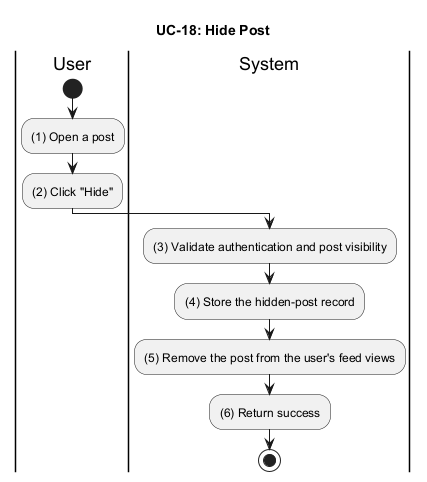
\includegraphics[width=0.8\textwidth]{./diagrams/activity_diagrams/UC_18_Hide_Post.png}
    \caption{Activity Diagram for UC-18}
    \label{fig:ad_uc18}
\end{figure}


\begin{longtblr}[
    caption = {Business Rules for UC-18 - Hide Post},
    label = {tab:uc18_business_rules}
]{
    width=\textwidth,
    hlines,
    vlines,
    rowhead = 1,
    rows = {valign=m, cmd=\nopagebreak},
    row{1} = {font=\bfseries, halign=c},
    colspec = {
        Q[c,1.5cm]
        Q[c,1.5cm]
        Q[l,11cm]
    }
}
\textbf{Activity} & \textbf{BR Code} & \textbf{Description} \\

(3--6) & BR1 &
\textbf{Hide the Post:}
\begin{itemize}
    \item The system validates authentication and confirms that the requester is the post author.
    \item The system marks the post as hidden using \textbf{\textit{HidePost()}}.
    \item The system removes the post from the user's visible feed views.
\end{itemize} \\
\end{longtblr}


\subsection{UC-19 - Manage Drafts}
\begin{table}[H]
\centering
\begin{tblr}{
    width=\textwidth,
    hlines,
    vlines,
    rows = {valign=m},
    colspec = {Q[l,3cm] Q[l,11cm]}
}
\textbf{Name} & Manage Drafts \\
\textbf{Description} & This use case describes how a user saves unfinished posts as drafts and publishes them later. \\
\textbf{Actor} & User \\
\textbf{Trigger} & When the user saves, edits, opens, or publishes a draft. \\
\textbf{Pre-condition} & The user is logged in to the system. \newline The user has draft access. \\
\textbf{Post-condition} & The draft is saved, updated, or deleted after publishing. \newline A published draft becomes a normal post. \\
\end{tblr}
\caption{Use Case Specification - Manage Drafts}
\end{table}


\begin{figure}[H]
    \centering
    
\includegraphics[width=0.8\textwidth]{./diagrams/activity_diagrams/UC_19_Manage_Drafts.png}
    \caption{Activity Diagram for UC-19}
    \label{fig:ad_uc19}
\end{figure}


\begin{longtblr}[
    caption = {Business Rules for UC-19 - Manage Drafts},
    label = {tab:uc19_business_rules}
]{
    width=\textwidth,
    hlines,
    vlines,
    rowhead = 1,
    rows = {valign=m, cmd=\nopagebreak},
    row{1} = {font=\bfseries, halign=c},
    colspec = {
        Q[c,1.5cm]
        Q[c,1.5cm]
        Q[l,11cm]
    }
}
\textbf{Activity} & \textbf{BR Code} & \textbf{Description} \\

(2--3) & BR1 &
\textbf{Load Drafts:}
\begin{itemize}
    \item The system loads the authenticated user's draft list using \textbf{\textit{GetDraftsByAuthor()}}.
    \item The system returns drafts together with pagination data.
\end{itemize} \\

(6--7) & BR2 &
\textbf{Create or Update Draft:}
\begin{itemize}
    \item The system validates draft ownership before saving changes.
    \item The system stores the draft via \textbf{\textit{CreateDraft()}} or \textbf{\textit{UpdateDraft()}}.
    \item The system updates text, images, videos, poll data, tags, and community selection on the draft record.
\end{itemize} \\

(8--10) & BR3 &
\textbf{Publish or Delete Draft:}
\begin{itemize}
    \item The system checks required fields before publishing a draft.
    \item The system creates the post from the draft using \textbf{\textit{PublishDraft()}}.
    \item After successful publishing, the system deletes the draft record.
\end{itemize} \\
\end{longtblr}


\subsection{UC-20 - Private Messaging}
\begin{table}[H]
\centering
\begin{tblr}{
    width=\textwidth,
    hlines,
    vlines,
    rows = {valign=m},
    colspec = {Q[l,3cm] Q[l,11cm]}
}
\textbf{Name} & Private Messaging \\
\textbf{Description} & This use case describes how users exchange instant one-to-one messages through the messaging system. \\
\textbf{Actor} & User \\
\textbf{Trigger} & When the user opens a conversation and sends a message. \\
\textbf{Pre-condition} & The user is logged in to the system. \newline The conversation channel exists and is accessible. \\
\textbf{Post-condition} & The message is delivered to the conversation members. \newline The channel read state is updated. \\
\end{tblr}
\caption{Use Case Specification - Private Messaging}
\end{table}


\begin{figure}[H]
    \centering
    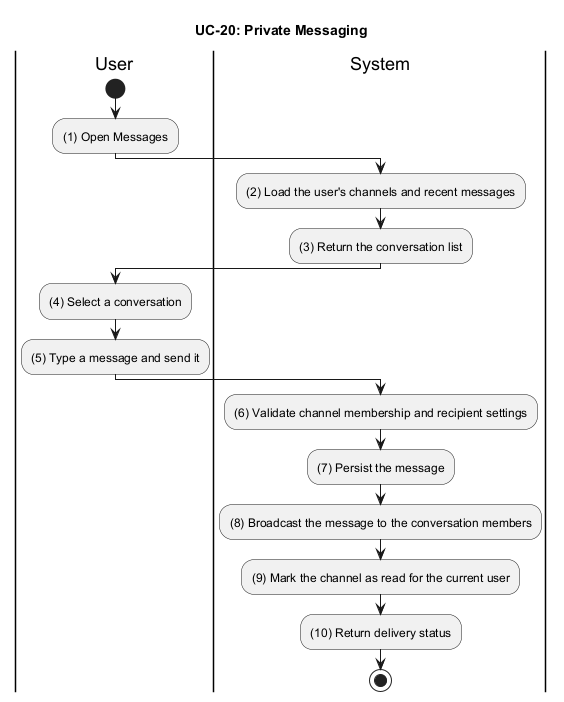
\includegraphics[width=0.8\textwidth]{./diagrams/activity_diagrams/UC_20_Private_Messaging.png}
    \caption{Activity Diagram for UC-20}
    \label{fig:ad_uc20}
\end{figure}


\begin{longtblr}[
    caption = {Business Rules for UC-20 - Private Messaging},
    label = {tab:uc20_business_rules}
]{
    width=\textwidth,
    hlines,
    vlines,
    rowhead = 1,
    rows = {valign=m, cmd=\nopagebreak},
    row{1} = {font=\bfseries, halign=c},
    colspec = {
        Q[c,1.5cm]
        Q[c,1.5cm]
        Q[l,11cm]
    }
}
\textbf{Activity} & \textbf{BR Code} & \textbf{Description} \\

(2--3) & BR1 &
\textbf{Load Conversations:}
\begin{itemize}
    \item The system loads the authenticated user's channels using \textbf{\textit{GetChannelsByUserID()}}.
    \item The system returns the conversation list and recent message state.
\end{itemize} \\

(4--10) & BR2 &
\textbf{Send and Deliver Message:}
\begin{itemize}
    \item The system validates that the sender is a channel member and that the recipients allow direct messages.
    \item The system persists the message and broadcasts it to the other channel members.
    \item The system marks the channel as read for the active user using \textbf{\textit{MarkChannelAsRead()}}.
\end{itemize} \\
\end{longtblr}


\subsection{UC-21 - Manage Notifications}
\begin{table}[H]
\centering
\begin{tblr}{
    width=\textwidth,
    hlines,
    vlines,
    rows = {valign=m},
    colspec = {Q[l,3cm] Q[l,11cm]}
}
\textbf{Name} & Manage Notifications \\
\textbf{Description} & This use case describes how a user views and clears system notifications. \\
\textbf{Actor} & User \\
\textbf{Trigger} & When the user opens the notifications page or marks notifications as read. \\
\textbf{Pre-condition} & The user is logged in to the system. \newline Notifications exist for the account. \\
\textbf{Post-condition} & The selected notifications are marked as read or deleted. \newline The notification list is refreshed. \\
\end{tblr}
\caption{Use Case Specification - Manage Notifications}
\end{table}


\begin{figure}[H]
    \centering
    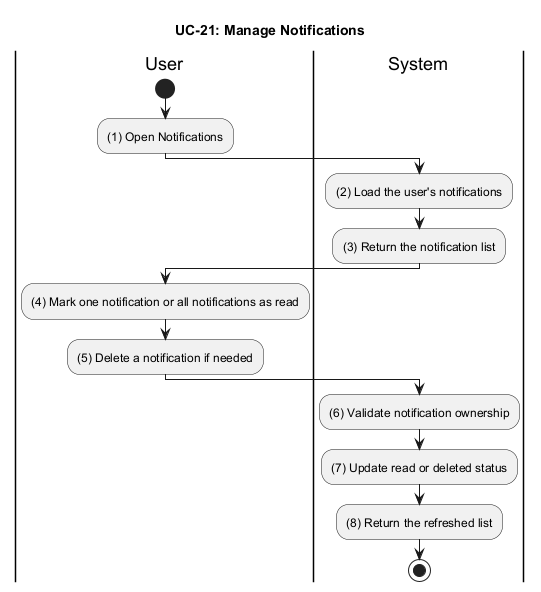
\includegraphics[width=0.8\textwidth]{./diagrams/activity_diagrams/UC_21_Manage_Notifications.png}
    \caption{Activity Diagram for UC-21}
    \label{fig:ad_uc21}
\end{figure}


\begin{longtblr}[
    caption = {Business Rules for UC-21 - Manage Notifications},
    label = {tab:uc21_business_rules}
]{
    width=\textwidth,
    hlines,
    vlines,
    rowhead = 1,
    rows = {valign=m, cmd=\nopagebreak},
    row{1} = {font=\bfseries, halign=c},
    colspec = {
        Q[c,1.5cm]
        Q[c,1.5cm]
        Q[l,11cm]
    }
}
\textbf{Activity} & \textbf{BR Code} & \textbf{Description} \\

(2--3) & BR1 &
\textbf{Load Notifications:}
\begin{itemize}
    \item The system loads notifications for \textbf{recipientID} using \textbf{\textit{GetNotifications()}}.
    \item The system returns the notification list with pagination data.
\end{itemize} \\

(4--8) & BR2 &
\textbf{Update Notification State:}
\begin{itemize}
    \item The system validates notification ownership before changing any record.
    \item If the user marks all notifications as read, the system updates them using \textbf{\textit{MarkAllAsRead()}}.
    \item If the user marks a single notification as read, the system validates \textbf{notificationID}, converts it to an object ID, and updates it using \textbf{\textit{MarkAsRead()}}.
    \item If the user deletes a notification, the system validates \textbf{notificationID} and removes it using \textbf{\textit{DeleteNotification()}}.
    \item The system returns the refreshed notification list after the update.
\end{itemize} \\
\end{longtblr}


\subsection{UC-22 - Report Violation}
\begin{table}[H]
\centering
\begin{tblr}{
    width=\textwidth,
    hlines,
    vlines,
    rows = {valign=m},
    colspec = {Q[l,3cm] Q[l,11cm]}
}
\textbf{Name} & Report Violation \\
\textbf{Description} & This use case describes how a user reports inappropriate content or behavior for review. \\
\textbf{Actor} & User \\
\textbf{Trigger} & When the user submits a report form. \\
\textbf{Pre-condition} & The user is logged in to the system. \newline The reported target is available. \\
\textbf{Post-condition} & The report is stored in the moderation queue. \newline The report can be reviewed by moderators or admins. \\
\end{tblr}
\caption{Use Case Specification - Report Violation}
\end{table}


\begin{figure}[H]
    \centering
    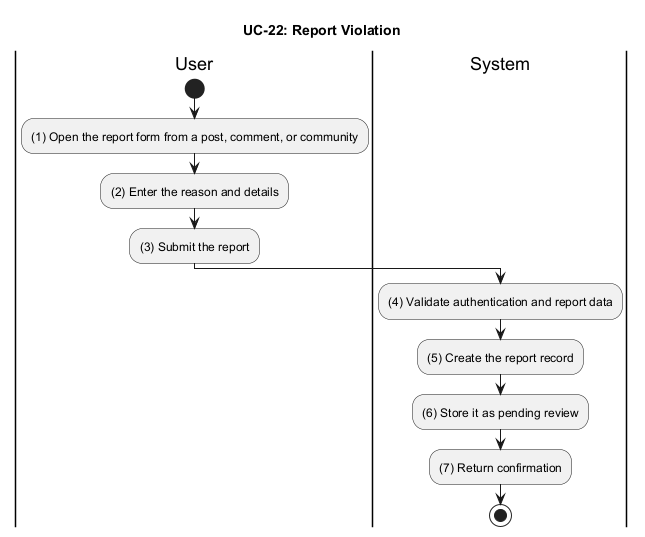
\includegraphics[width=0.8\textwidth]{./diagrams/activity_diagrams/UC_22_Report_Violation.png}
    \caption{Activity Diagram for UC-22}
    \label{fig:ad_uc22}
\end{figure}


\begin{longtblr}[
    caption = {Business Rules for UC-22 - Report Violation},
    label = {tab:uc22_business_rules}
]{
    width=\textwidth,
    hlines,
    vlines,
    rowhead = 1,
    rows = {valign=m, cmd=\nopagebreak},
    row{1} = {font=\bfseries, halign=c},
    colspec = {
        Q[c,1.5cm]
        Q[c,1.5cm]
        Q[l,11cm]
    }
}
\textbf{Activity} & \textbf{BR Code} & \textbf{Description} \\

(1--3) & BR1 &
\textbf{Validate Report Submission:}
\begin{itemize}
    \item The system checks that the user is authenticated.
    \item The system validates the submitted \textbf{reason} and \textbf{details} in \textbf{\textit{ReportPost()}}.
    \item The system checks that the target post exists and that \textbf{reporterID} is not the post author.
\end{itemize} \\

(4--7) & BR2 &
\textbf{Create Report Record:}
\begin{itemize}
    \item The system creates a new report with \textbf{Create()} on the report repository.
    \item The system stores the report as pending review.
    \item The system returns a confirmation message after the report is saved.
\end{itemize} \\
\end{longtblr}


\subsection{UC-23 - Create Community}
\begin{table}[H]
\centering
\begin{tblr}{
    width=\textwidth,
    hlines,
    vlines,
    rows = {valign=m},
    colspec = {Q[l,3cm] Q[l,11cm]}
}
\textbf{Name} & Create Community \\
\textbf{Description} & This use case describes how a user creates a new community and becomes its owner. \\
\textbf{Actor} & User \\
\textbf{Trigger} & When the user submits the create community form. \\
\textbf{Pre-condition} & The user is logged in to the system. \newline The community name is available and valid. \\
\textbf{Post-condition} & The community is created successfully. \newline The creator becomes the owner and first member. \\
\end{tblr}
\caption{Use Case Specification - Create Community}
\end{table}


\begin{figure}[H]
    \centering
    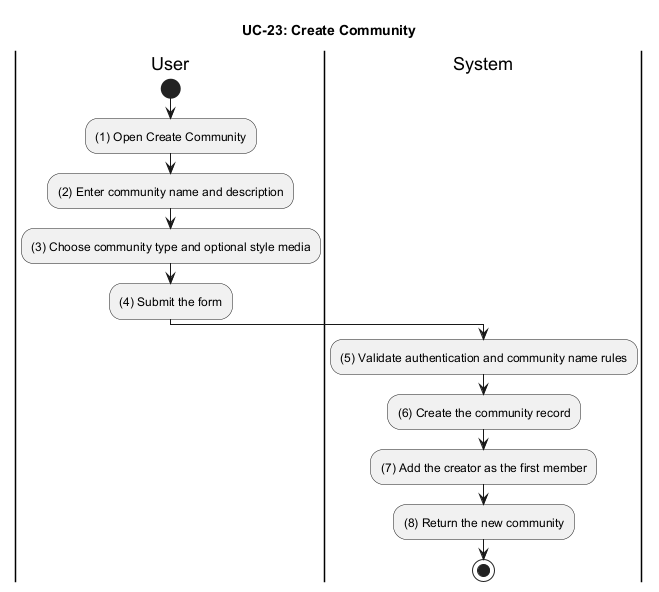
\includegraphics[width=0.8\textwidth]{./diagrams/activity_diagrams/UC_23_Create_Community.png}
    \caption{Activity Diagram for UC-23}
    \label{fig:ad_uc23}
\end{figure}


\begin{longtblr}[
    caption = {Business Rules for UC-23 - Create Community},
    label = {tab:uc23_business_rules}
]{
    width=\textwidth,
    hlines,
    vlines,
    rowhead = 1,
    rows = {valign=m, cmd=\nopagebreak},
    row{1} = {font=\bfseries, halign=c},
    colspec = {
        Q[c,1.5cm]
        Q[c,1.5cm]
        Q[l,11cm]
    }
}
\textbf{Activity} & \textbf{BR Code} & \textbf{Description} \\

(1--4) & BR1 &
\textbf{Validate Community Input:}
\begin{itemize}
    \item The system checks that the user is authenticated.
    \item The system validates the submitted community fields, especially \textbf{name} in \textbf{\textit{CreateCommunity()}}.
    \item The system rejects duplicate community names with a community-name-exists error.
\end{itemize} \\

(5--8) & BR2 &
\textbf{Create Community and Initial Membership:}
\begin{itemize}
    \item The system creates the community record with \textbf{\textit{CreateCommunity()}}.
    \item The system adds the creator as the first member by creating a membership record.
    \item The system returns the new community after persistence succeeds.
\end{itemize} \\
\end{longtblr}


\subsection{UC-24 - Approve / Reject Post}
\begin{table}[H]
\centering
\begin{tblr}{
    width=\textwidth,
    hlines,
    vlines,
    rows = {valign=m},
    colspec = {Q[l,3cm] Q[l,11cm]}
}
\textbf{Name} & Approve / Reject Post \\
\textbf{Description} & This use case describes how a moderator reviews pending or edited posts and decides whether to publish them. \\
\textbf{Actor} & Moderator \\
\textbf{Trigger} & When the moderator opens the moderation queue and chooses approve or reject. \\
\textbf{Pre-condition} & The moderator is logged in to the system. \newline The target post is pending review or edited. \\
\textbf{Post-condition} & The post is approved or rejected. \newline The moderation result is stored and reflected in the community. \\
\end{tblr}
\caption{Use Case Specification - Approve / Reject Post}
\end{table}


\begin{figure}[H]
    \centering
    
\includegraphics[width=0.8\textwidth]{./diagrams/activity_diagrams/UC_24_Approve_Reject_Post.png}
    \caption{Activity Diagram for UC-24}
    \label{fig:ad_uc24}
\end{figure}

\begin{longtblr}[
    caption = {Business Rules for UC-24 - Approve / Reject Post},
    label = {tab:uc24_business_rules}
]{
    width=\textwidth,
    hlines,
    vlines,
    rowhead = 1,
    rows = {valign=m, cmd=\nopagebreak},
    row{1} = {font=\bfseries, halign=c},
    colspec = {
        Q[c,1.5cm]
        Q[c,1.5cm]
        Q[l,11cm]
    }
}
\textbf{Activity} & \textbf{BR Code} & \textbf{Description} \\

(1--4) & BR1 &
\textbf{Prepare Moderation Decision:}
\begin{itemize}
    \item The system loads the moderation queue using \textbf{\textit{GetPendingPosts()}} and \textbf{\textit{GetEditedPosts()}}.
    \item The system validates that the requester has moderator access.
    \item The system checks that the selected post belongs to the current community and is still pending moderation.
\end{itemize} \\

(5--8) & BR2 &
\textbf{Apply Moderation Result:}
\begin{itemize}
    \item The system updates the post using \textbf{\textit{ModeratePost()}}.
    \item If the moderator approves the post, the system sets the moderation status to approved and publishes the post to the community.
    \item If the moderator rejects the post, the system sets the moderation status to rejected and stores the rejection \textbf{reason}.
    \item The system returns the moderation result to the caller.
\end{itemize} \\
\end{longtblr}


\subsection{UC-25 - Ban / Mute User}
\begin{table}[H]
\centering
\begin{tblr}{
    width=\textwidth,
    hlines,
    vlines,
    rows = {valign=m},
    colspec = {Q[l,3cm] Q[l,11cm]}
}
\textbf{Name} & Ban / Mute User \\
\textbf{Description} & This use case describes how a moderator restricts a user's participation in a community. \\
\textbf{Actor} & Moderator \\
\textbf{Trigger} & When the moderator chooses to ban or mute a user. \\
\textbf{Pre-condition} & The moderator is logged in to the system. \newline The target user belongs to the community. \\
\textbf{Post-condition} & The ban or mute restriction is stored. \newline The user is prevented from performing the restricted actions. \\
\end{tblr}
\caption{Use Case Specification - Ban / Mute User}
\end{table}


\begin{figure}[H]
    \centering
    
\includegraphics[width=0.8\textwidth]{./diagrams/activity_diagrams/UC_25_Ban_Mute_User.png}
    \caption{Activity Diagram for UC-25}
    \label{fig:ad_uc25}
\end{figure}


\begin{longtblr}[
    caption = {Business Rules for UC-25 - Ban / Mute User},
    label = {tab:uc25_business_rules}
]{
    width=\textwidth,
    hlines,
    vlines,
    rowhead = 1,
    rows = {valign=m, cmd=\nopagebreak},
    row{1} = {font=\bfseries, halign=c},
    colspec = {
        Q[c,1.5cm]
        Q[c,1.5cm]
        Q[l,11cm]
    }
}
\textbf{Activity} & \textbf{BR Code} & \textbf{Description} \\

(1--4) & BR1 &
\textbf{Validate Restriction Request:}
\begin{itemize}
    \item The system checks that the requester has moderator access.
    \item The system validates the target \textbf{userID}, \textbf{communityID}, \textbf{Type}, \textbf{Reason}, and \textbf{LengthDays}.
    \item The system accepts only the \textbf{banned} or \textbf{muted} restriction type.
\end{itemize} \\

(5--7) & BR2 &
\textbf{Store Ban or Mute Record:}
\begin{itemize}
    \item The system calculates the expiration timestamp from \textbf{LengthDays}.
    \item The system creates a community ban record through \textbf{\textit{BanUser()}}.
    \item The system stores either a ban or mute entry based on \textbf{Type} and returns the updated restriction state.
\end{itemize} \\
\end{longtblr}


\subsection{UC-26 - Configure Community}
\begin{table}[H]
\centering
\begin{tblr}{
    width=\textwidth,
    hlines,
    vlines,
    rows = {valign=m},
    colspec = {Q[l,3cm] Q[l,11cm]}
}
\textbf{Name} & Configure Community \\
\textbf{Description} & This use case describes how a community owner updates rules, privacy, and appearance settings. \\
\textbf{Actor} & Owner \\
\textbf{Trigger} & When the owner opens the community settings page and saves changes. \\
\textbf{Pre-condition} & The owner is logged in to the system. \newline The owner has permission to manage the community. \\
\textbf{Post-condition} & The community configuration is updated. \newline The new settings are applied to the community. \\
\end{tblr}
\caption{Use Case Specification - Configure Community}
\end{table}


\begin{figure}[H]
    \centering
    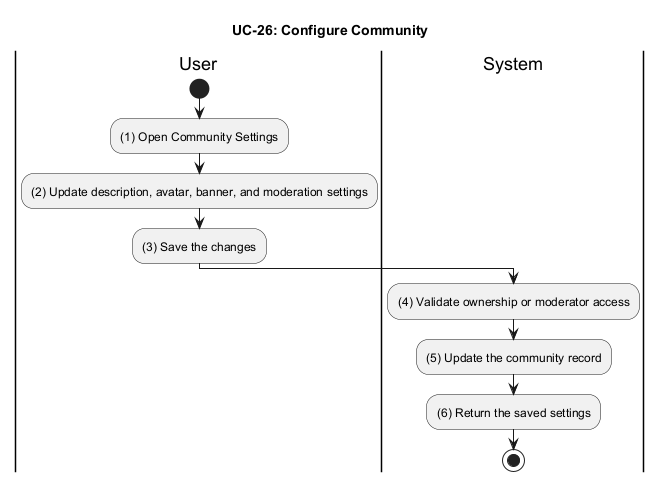
\includegraphics[width=0.8\textwidth]{./diagrams/activity_diagrams/UC_26_Configure_Community.png}
    \caption{Activity Diagram for UC-26}
    \label{fig:ad_uc26}
\end{figure}


\begin{longtblr}[
    caption = {Business Rules for UC-26 - Configure Community},
    label = {tab:uc26_business_rules}
]{
    width=\textwidth,
    hlines,
    vlines,
    rowhead = 1,
    rows = {valign=m, cmd=\nopagebreak},
    row{1} = {font=\bfseries, halign=c},
    colspec = {
        Q[c,1.5cm]
        Q[c,1.5cm]
        Q[l,11cm]
    }
}
\textbf{Activity} & \textbf{BR Code} & \textbf{Description} \\

(1--3) & BR1 &
\textbf{Validate Community Access:}
\begin{itemize}
    \item The system checks that the requester has moderator access for the community.
    \item The system validates the incoming community settings before saving them.
\end{itemize} \\

(4--6) & BR2 &
\textbf{Persist Community Settings:}
\begin{itemize}
    \item The system updates the community record using \textbf{\textit{UpdateCommunity()}}.
    \item The system saves the description, avatar, banner, and moderation settings.
    \item The system returns the saved community settings.
\end{itemize} \\
\end{longtblr}


\subsection{UC-27 - Assign Roles}
\begin{table}[H]
\centering
\begin{tblr}{
    width=\textwidth,
    hlines,
    vlines,
    rows = {valign=m},
    colspec = {Q[l,3cm] Q[l,11cm]}
}
\textbf{Name} & Assign Roles \\
\textbf{Description} & This use case describes how a community owner appoints moderators or other roles for members. \\
\textbf{Actor} & Owner \\
\textbf{Trigger} & When the owner invites or activates a role for another member. \\
\textbf{Pre-condition} & The owner is logged in to the system. \newline The target member belongs to the community. \\
\textbf{Post-condition} & The role assignment is stored successfully. \newline The target member gains the new permissions. \\
\end{tblr}
\caption{Use Case Specification - Assign Roles}
\end{table}


\begin{figure}[H]
    \centering
    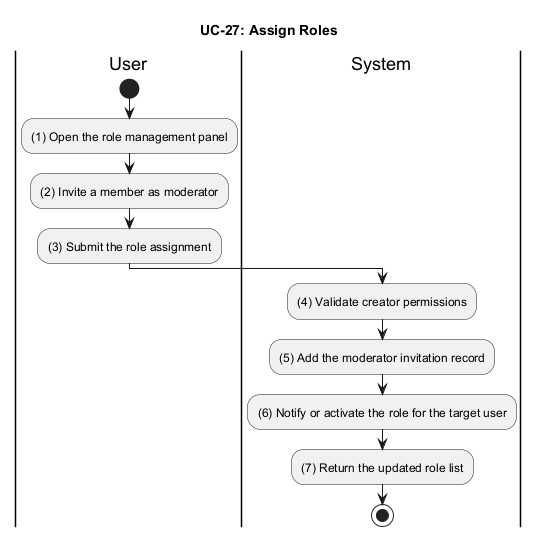
\includegraphics[width=0.8\textwidth]{./diagrams/activity_diagrams/UC_27_Assign_Roles.png}
    \caption{Activity Diagram for UC-27}
    \label{fig:ad_uc27}
\end{figure}


\begin{longtblr}[
    caption = {Business Rules for UC-27 - Assign Roles},
    label = {tab:uc27_business_rules}
]{
    width=\textwidth,
    hlines,
    vlines,
    rowhead = 1,
    rows = {valign=m, cmd=\nopagebreak},
    row{1} = {font=\bfseries, halign=c},
    colspec = {
        Q[c,1.5cm]
        Q[c,1.5cm]
        Q[l,11cm]
    }
}
\textbf{Activity} & \textbf{BR Code} & \textbf{Description} \\

(1--3) & BR1 &
\textbf{Validate Role Assignment:}
\begin{itemize}
    \item The system checks that the requester is the community creator.
    \item The system validates the moderator assignment payload, including \textbf{CommunityID} and \textbf{AddedModerator}.
\end{itemize} \\

(4--7) & BR2 &
\textbf{Add and Activate Moderator Role:}
\begin{itemize}
    \item The system creates the moderator invitation or assignment record using \textbf{\textit{AddModerator()}}.
    \item The system activates the moderator role for the target user using \textbf{\textit{ActivateModerator()}} when the role becomes active.
    \item The system returns the updated moderator list.
\end{itemize} \\
\end{longtblr}


\subsection{UC-28 - Handle Global Reports}
\begin{table}[H]
\centering
\begin{tblr}{
    width=\textwidth,
    hlines,
    vlines,
    rows = {valign=m},
    colspec = {Q[l,3cm] Q[l,11cm]}
}
\textbf{Name} & Handle Global Reports \\
\textbf{Description} & This use case describes how a system admin reviews and acts on platform-wide violation reports. \\
\textbf{Actor} & System Admin \\
\textbf{Trigger} & When the admin opens the global reports dashboard. \\
\textbf{Pre-condition} & The admin is logged in to the system. \newline There are reports available for review. \\
\textbf{Post-condition} & The selected reports are reviewed or deleted. \newline The report queue is updated. \\
\end{tblr}
\caption{Use Case Specification - Handle Global Reports}
\end{table}


\begin{figure}[H]
    \centering
    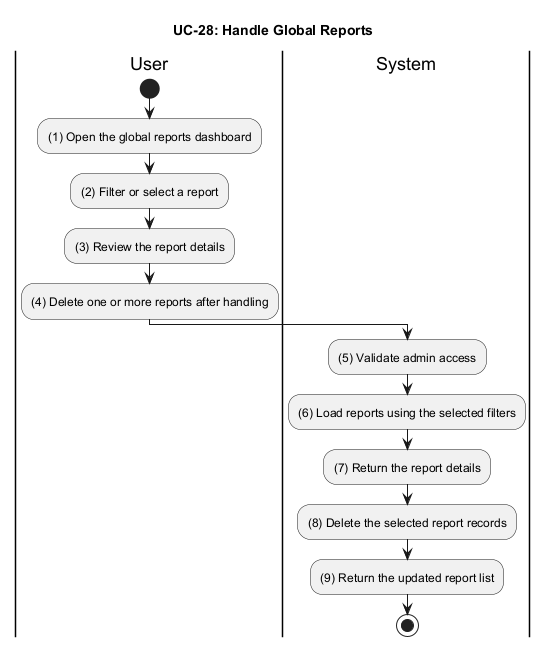
\includegraphics[width=0.8\textwidth]{./diagrams/activity_diagrams/UC_28_Handle_Global_Reports.png}
    \caption{Activity Diagram for UC-28}
    \label{fig:ad_uc28}
\end{figure}


\begin{longtblr}[
    caption = {Business Rules for UC-28 - Handle Global Reports},
    label = {tab:uc28_business_rules}
]{
    width=\textwidth,
    hlines,
    vlines,
    rowhead = 1,
    rows = {valign=m, cmd=\nopagebreak},
    row{1} = {font=\bfseries, halign=c},
    colspec = {
        Q[c,1.5cm]
        Q[c,1.5cm]
        Q[l,11cm]
    }
}
\textbf{Activity} & \textbf{BR Code} & \textbf{Description} \\

(1--3) & BR1 &
\textbf{Load and Inspect Reports:}
\begin{itemize}
    \item The system checks that the requester is an admin.
    \item The system loads filtered reports using \textbf{\textit{GetReportsFilter()}}.
    \item The system allows the admin to inspect a single report using \textbf{\textit{GetReportByID()}}.
\end{itemize} \\

(4--9) & BR2 &
\textbf{Delete Handled Reports:}
\begin{itemize}
    \item The system deletes a single report using \textbf{\textit{DeleteReport()}} or multiple reports using \textbf{\textit{DeleteReports()}}.
    \item The system validates that the admin is allowed to delete the selected report records.
    \item The system rejects an empty batch request.
    \item The system returns the updated report list after deletion.
\end{itemize} \\
\end{longtblr}


\subsection{UC-29 - Manage Platform}
\begin{table}[H]
\centering
\begin{tblr}{
    width=\textwidth,
    hlines,
    vlines,
    rows = {valign=m},
    colspec = {Q[l,3cm] Q[l,11cm]}
}
\textbf{Name} & Manage Platform \\
\textbf{Description} & This use case describes how a system admin manages users and communities globally. \\
\textbf{Actor} & System Admin \\
\textbf{Trigger} & When the admin opens the platform management area and selects a target entity. \\
\textbf{Pre-condition} & The admin is logged in to the system. \newline The admin has global management privileges. \\
\textbf{Post-condition} & The selected user or community is banned or unbanned. \newline The platform state is updated accordingly. \\
\end{tblr}
\caption{Use Case Specification - Manage Platform}
\end{table}


\begin{figure}[H]
    \centering
    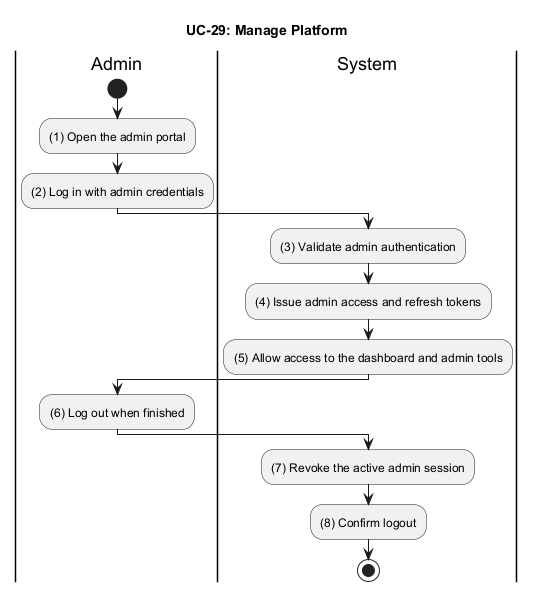
\includegraphics[width=0.8\textwidth]{./diagrams/activity_diagrams/UC_29_Manage_Platform.png}
    \caption{Activity Diagram for UC-29}
    \label{fig:ad_uc29}
\end{figure}


\begin{longtblr}[
    caption = {Business Rules for UC-29 - Manage Platform},
    label = {tab:uc29_business_rules}
]{
    width=\textwidth,
    hlines,
    vlines,
    rowhead = 1,
    rows = {valign=m, cmd=\nopagebreak},
    row{1} = {font=\bfseries, halign=c},
    colspec = {
        Q[c,1.5cm]
        Q[c,1.5cm]
        Q[l,11cm]
    }
}
\textbf{Activity} & \textbf{BR Code} & \textbf{Description} \\

(1--5) & BR1 &
\textbf{Authenticate Admin Access:}
\begin{itemize}
    \item The system checks the admin credentials and requires the user to have the admin role.
    \item The system rejects banned or deleted admin accounts.
    \item The system verifies the password for local accounts and issues access and refresh tokens using \textbf{\textit{AdminLogin()}}.
\end{itemize} \\

(6--8) & BR2 &
\textbf{End the Admin Session:}
\begin{itemize}
    \item The system revokes the active admin session using \textbf{\textit{AdminLogout()}}.
    \item The system invalidates the stored access and refresh tokens when token revocation is available.
    \item The system confirms logout after session cleanup.
\end{itemize} \\
\end{longtblr}


\subsection{UC-30 - View Analytics}
\begin{table}[H]
\centering
\begin{tblr}{
    width=\textwidth,
    hlines,
    vlines,
    rows = {valign=m},
    colspec = {Q[l,3cm] Q[l,11cm]}
}
\textbf{Name} & View Analytics \\
\textbf{Description} & This use case describes how a system admin reviews platform usage and performance metrics. \\
\textbf{Actor} & System Admin \\
\textbf{Trigger} & When the admin opens the analytics dashboard. \\
\textbf{Pre-condition} & The admin is logged in to the system. \newline Analytics data is available for the selected period. \\
\textbf{Post-condition} & The analytics dashboard is displayed with current metrics. \newline The admin can review user, content, and moderation statistics. \\
\end{tblr}
\caption{Use Case Specification - View Analytics}
\end{table}


\begin{figure}[H]
    \centering
    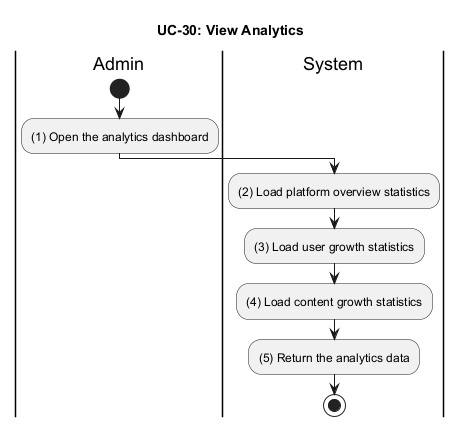
\includegraphics[width=0.8\textwidth]{./diagrams/activity_diagrams/UC_30_View_Analytics.png}
    \caption{Activity Diagram for UC-30}
    \label{fig:ad_uc30}
\end{figure}


\begin{longtblr}[
    caption = {Business Rules for UC-30 - View Analytics},
    label = {tab:uc30_business_rules}
]{
    width=\textwidth,
    hlines,
    vlines,
    rowhead = 1,
    rows = {valign=m, cmd=\nopagebreak},
    row{1} = {font=\bfseries, halign=c},
    colspec = {
        Q[c,1.5cm]
        Q[c,1.5cm]
        Q[l,11cm]
    }
}
\textbf{Activity} & \textbf{BR Code} & \textbf{Description} \\

(1--5) & BR1 &
\textbf{Load Platform Analytics:}
\begin{itemize}
    \item The system checks that the requester is an admin.
    \item The system loads platform overview data using \textbf{\textit{GetPlatformOverview()}}.
    \item The system aggregates user, content, and moderation statistics from the backend services.
\end{itemize} \\

(2--5) & BR2 &
\textbf{Return Analytics Breakdowns:}
\begin{itemize}
    \item The system returns user growth and content growth data using \textbf{\textit{GetUserStats()}} and \textbf{\textit{GetContentStats()}}.
    \item The system includes the current overview snapshot in the analytics response.
\end{itemize} \\
\end{longtblr}

\section{Data Requirements}

\subsection{Logical Data Model}

\begin{figure}[H]
    \centering
    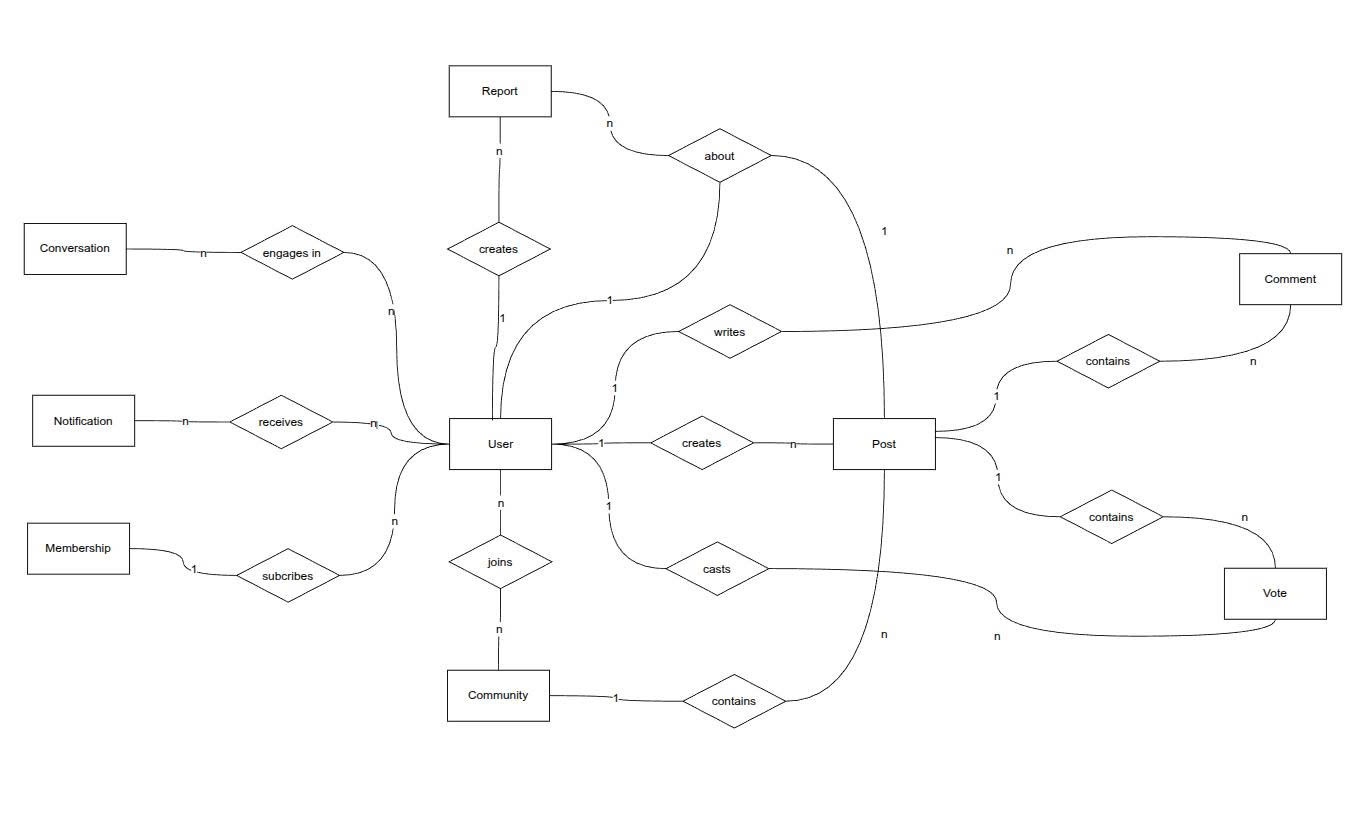
\includegraphics[width=\textwidth]{./diagrams/Partial data model for LKForum.jpg}
    \caption{Logical Data Model for LKForum}
    \label{fig:data_model_lkforum}
\end{figure}

\subsection{Data Dictionary}

\subsubsection{Authentication and User Profile Models}

\begin{longtblr}[
    caption = {User},
    label = {tab:data_dictionary_user}
]{
    width=\textwidth,
    hlines,
    vlines,
    rows = {valign=m},
    row{1} = {font=\bfseries, halign=c},
    colspec = {Q[l,2.8cm] Q[l,4.5cm] Q[c,2.5cm] Q[c,1.5cm] Q[l,4.2cm]}
}
\textbf{Data Element} & \textbf{Description} & \textbf{Composition / Data Type} & \textbf{Length} & \textbf{Values} \\

ID & Unique identifier of a user. & objectId & 24 & System-generated, unique. \\
Username & Display name used to identify a user account. & string & -- & Must be unique within the platform. \\
Email & Email address used for authentication and contact. & string & -- & Must be unique and valid. \\
Reputation & User reputation score. & integer & -- & System-maintained counter. \\
Password & Hashed password for a local account. & string & -- & Stored only for local providers. \\
Provider & Authentication source for a user account. & enum & -- & local, google \\
ProviderID & External account identifier returned by the provider. & string & -- & Used for third-party login linkage. \\
Role & Platform-wide role of the user. & enum & -- & user, admin \\
RoleContent & Role-specific data attached to the user account. & object & -- & Contains user or admin sub-document data. \\
Settings & User preference configuration. & object & -- & Contains appearance, notification, privacy, and content settings. \\
IsVerified & Indicates whether the account has been verified. & boolean & -- & true, false \\
IsBanned & Indicates whether the account is currently banned. & boolean & -- & true, false \\
BanUntil & Timestamp when a ban expires, if any. & timestamp & -- & Null means permanent ban. \\
BanReason & Reason recorded for a ban action. & string & -- & Optional free text. \\
CreatedAt & Timestamp when the record was created. & timestamp & -- & System-generated. \\
DeletedAt & Timestamp for soft-deleted records. & timestamp & -- & Null when not deleted. \\
\end{longtblr}

\begin{longtblr}[
    caption = {RoleContent},
    label = {tab:data_dictionary_role_content}
]{
    width=\textwidth,
    hlines,
    vlines,
    rows = {valign=m},
    row{1} = {font=\bfseries, halign=c},
    colspec = {Q[l,2.8cm] Q[l,4.5cm] Q[c,2.5cm] Q[c,1.5cm] Q[l,4.2cm]}
}
\textbf{Data Element} & \textbf{Description} & \textbf{Composition / Data Type} & \textbf{Length} & \textbf{Values} \\

AsUser & User-specific profile data. & object & -- & See UserRoleContent table. \\
AsAdmin & Admin-specific profile data. & object & -- & See AdminRoleContent table. \\
\end{longtblr}

\begin{longtblr}[
    caption = {UserRoleContent},
    label = {tab:data_dictionary_user_role_content}
]{
    width=\textwidth,
    hlines,
    vlines,
    rows = {valign=m},
    row{1} = {font=\bfseries, halign=c},
    colspec = {Q[l,2.8cm] Q[l,4.5cm] Q[c,2.5cm] Q[c,1.5cm] Q[l,4.2cm]}
}
\textbf{Data Element} & \textbf{Description} & \textbf{Composition / Data Type} & \textbf{Length} & \textbf{Values} \\

Avatar & Profile image. & object & -- & See Image table. \\
Cover & Cover image. & object & -- & See Image table. \\
Bio & Short biography. & string & -- & User-generated text. \\
Gender & Declared gender. & enum & -- & male, female, prefer_not_to_say \\
DateOfBirth & User date of birth. & timestamp & -- & Optional date value. \\
Location & Province or city. & enum & -- & One of the provinces defined in model/location.go. \\
Interests & List of user interests. & array[string] & -- & Values defined in model/interest.go. \\
SocialLinks & Collection of public social profiles. & object & -- & Website, Facebook, YouTube, GitHub links. \\
Stats & User activity statistics. & object & -- & Post, comment, and vote counters plus timestamps. \\
\end{longtblr}

\begin{longtblr}[
    caption = {SocialLinks},
    label = {tab:data_dictionary_social_links}
]{
    width=\textwidth,
    hlines,
    vlines,
    rows = {valign=m},
    row{1} = {font=\bfseries, halign=c},
    colspec = {Q[l,2.8cm] Q[l,4.5cm] Q[c,2.5cm] Q[c,1.5cm] Q[l,4.2cm]}
}
\textbf{Data Element} & \textbf{Description} & \textbf{Composition / Data Type} & \textbf{Length} & \textbf{Values} \\

Website & Personal website URL. & string & -- & Optional URL. \\
Facebook & Facebook profile URL. & string & -- & Optional URL. \\
YouTube & YouTube channel URL. & string & -- & Optional URL. \\
GitHub & GitHub profile URL. & string & -- & Optional URL. \\
\end{longtblr}

\begin{longtblr}[
    caption = {ActivityStats},
    label = {tab:data_dictionary_activity_stats}
]{
    width=\textwidth,
    hlines,
    vlines,
    rows = {valign=m},
    row{1} = {font=\bfseries, halign=c},
    colspec = {Q[l,2.8cm] Q[l,4.5cm] Q[c,2.5cm] Q[c,1.5cm] Q[l,4.2cm]}
}
\textbf{Data Element} & \textbf{Description} & \textbf{Composition / Data Type} & \textbf{Length} & \textbf{Values} \\

PostCount & Number of posts created. & integer & -- & System-maintained counter. \\
CommentCount & Number of comments created. & integer & -- & System-maintained counter. \\
TotalUpvotes & Total upvotes received. & integer & -- & System-maintained counter. \\
JoinedAt & Timestamp when the user joined. & timestamp & -- & System-generated. \\
LastActiveAt & Timestamp of the last activity. & timestamp & -- & System-generated. \\
\end{longtblr}

\begin{longtblr}[
    caption = {AdminRoleContent},
    label = {tab:data_dictionary_admin_role_content}
]{
    width=\textwidth,
    hlines,
    vlines,
    rows = {valign=m},
    row{1} = {font=\bfseries, halign=c},
    colspec = {Q[l,2.8cm] Q[l,4.5cm] Q[c,2.5cm] Q[c,1.5cm] Q[l,4.2cm]}
}
\textbf{Data Element} & \textbf{Description} & \textbf{Composition / Data Type} & \textbf{Length} & \textbf{Values} \\

Permissions & Admin capability list. & array[string] & -- & Permission names granted to the admin. \\
\end{longtblr}

\begin{longtblr}[
    caption = {UserSettings},
    label = {tab:data_dictionary_user_settings}
]{
    width=\textwidth,
    hlines,
    vlines,
    rows = {valign=m},
    row{1} = {font=\bfseries, halign=c},
    colspec = {Q[l,2.8cm] Q[l,4.5cm] Q[c,2.5cm] Q[c,1.5cm] Q[l,4.2cm]}
}
\textbf{Data Element} & \textbf{Description} & \textbf{Composition / Data Type} & \textbf{Length} & \textbf{Values} \\

Appearance & Visual preferences. & object & -- & See AppearanceSettings table. \\
Notifications & Notification preferences. & object & -- & See NotificationSettings table. \\
Privacy & Privacy preferences. & object & -- & See PrivacySettings table. \\
Content & Content filtering preferences. & object & -- & See ContentSettings table. \\
\end{longtblr}

\begin{longtblr}[
    caption = {AppearanceSettings},
    label = {tab:data_dictionary_appearance_settings}
]{
    width=\textwidth,
    hlines,
    vlines,
    rows = {valign=m},
    row{1} = {font=\bfseries, halign=c},
    colspec = {Q[l,2.8cm] Q[l,4.5cm] Q[c,2.5cm] Q[c,1.5cm] Q[l,4.2cm]}
}
\textbf{Data Element} & \textbf{Description} & \textbf{Composition / Data Type} & \textbf{Length} & \textbf{Values} \\

Theme & UI theme preference. & enum & -- & light, dark, auto \\
FontSize & UI font size preference. & enum & -- & small, medium, large \\
\end{longtblr}

\begin{longtblr}[
    caption = {NotificationSettings},
    label = {tab:data_dictionary_notification_settings}
]{
    width=\textwidth,
    hlines,
    vlines,
    rows = {valign=m},
    row{1} = {font=\bfseries, halign=c},
    colspec = {Q[l,2.8cm] Q[l,4.5cm] Q[c,2.5cm] Q[c,1.5cm] Q[l,4.2cm]}
}
\textbf{Data Element} & \textbf{Description} & \textbf{Composition / Data Type} & \textbf{Length} & \textbf{Values} \\

InAppEnabled & In-app notification toggle. & boolean & -- & true, false \\
EmailEnabled & Email notification toggle. & boolean & -- & true, false \\
NotifyOn-Comment & Notify on comments. & boolean & -- & true, false \\
NotifyOn-Mention & Notify on mentions. & boolean & -- & true, false \\
NotifyOnUpvote & Notify on upvotes. & boolean & -- & true, false \\
NotifyOnMessage & Notify on private messages. & boolean & -- & true, false \\
\end{longtblr}

\begin{longtblr}[
    caption = {PrivacySettings},
    label = {tab:data_dictionary_privacy_settings}
]{
    width=\textwidth,
    hlines,
    vlines,
    rows = {valign=m},
    row{1} = {font=\bfseries, halign=c},
    colspec = {Q[l,2.8cm] Q[l,4.5cm] Q[c,2.5cm] Q[c,1.5cm] Q[l,4.2cm]}
}
\textbf{Data Element} & \textbf{Description} & \textbf{Composition / Data Type} & \textbf{Length} & \textbf{Values} \\

ShowProfile & Controls whether a profile is public. & boolean & -- & true, false \\
ShowEmail & Controls whether email is visible on the profile. & boolean & -- & true, false \\
ShowPostHistory & Controls whether post history is visible. & boolean & -- & true, false \\
AllowDirect-Messages & Controls whether direct messages are allowed. & boolean & -- & true, false \\
AllowMentions & Controls whether mentions are allowed. & boolean & -- & true, false \\
\end{longtblr}

\begin{longtblr}[
    caption = {ContentSettings},
    label = {tab:data_dictionary_content_settings}
]{
    width=\textwidth,
    hlines,
    vlines,
    rows = {valign=m},
    row{1} = {font=\bfseries, halign=c},
    colspec = {Q[l,2.8cm] Q[l,4.5cm] Q[c,2.5cm] Q[c,1.5cm] Q[l,4.2cm]}
}
\textbf{Data Element} & \textbf{Description} & \textbf{Composition / Data Type} & \textbf{Length} & \textbf{Values} \\

AllowNSFW & Controls whether NSFW content is allowed. & boolean & -- & true, false \\
\end{longtblr}

\begin{longtblr}[
    caption = {Verification Records},
    label = {tab:data_dictionary_verification}
]{
    width=\textwidth,
    hlines,
    vlines,
    rows = {valign=m},
    row{1} = {font=\bfseries, halign=c},
    colspec = {Q[l,2.8cm] Q[l,4.5cm] Q[c,2.5cm] Q[c,1.5cm] Q[l,4.2cm]}
}
\textbf{Data Element} & \textbf{Description} & \textbf{Composition / Data Type} & \textbf{Length} & \textbf{Values} \\

EmailVerification-.ID & Unique identifier of an email verification record. & objectId & 24 & System-generated, unique. \\
EmailVerification-.Email & Email being verified. & string & -- & Must be unique and valid. \\
EmailVerification-.OTP & One-time password used for verification. & string & 6 & Six-digit numeric code. \\
EmailVerification-.OTPExpiresAt & Expiration timestamp for the OTP. & timestamp & -- & System-generated. \\
EmailVerification-.IsVerified & Indicates whether the OTP has already been verified. & boolean & -- & true, false \\
EmailVerification-.Nonce & Anti-replay token. & string & -- & System-generated random value. \\
EmailVerification-.CreatedAt & Timestamp when the record was created. & timestamp & -- & System-generated. \\
\end{longtblr}

\begin{longtblr}[
    caption = {PasswordReset},
    label = {tab:data_dictionary_password_reset}
]{
    width=\textwidth,
    hlines,
    vlines,
    rows = {valign=m},
    row{1} = {font=\bfseries, halign=c},
    colspec = {Q[l,2.8cm] Q[l,4.5cm] Q[c,2.5cm] Q[c,1.5cm] Q[l,4.2cm]}
}
\textbf{Data Element} & \textbf{Description} & \textbf{Composition / Data Type} & \textbf{Length} & \textbf{Values} \\

PasswordReset-.ID & Unique identifier of a password reset record. & objectId & 24 & System-generated, unique. \\
PasswordReset-.Email & Email being reset. & string & -- & Must be unique and valid. \\
PasswordReset-.OTP & One-time password used for reset. & string & 6 & Six-digit numeric code. \\
PasswordReset-.OTPExpiresAt & Expiration timestamp for the OTP. & timestamp & -- & System-generated. \\
PasswordReset-.IsVerified & Indicates whether the OTP has already been verified. & boolean & -- & true, false \\
PasswordReset-.Nonce & Anti-replay token. & string & -- & System-generated random value. \\
PasswordReset-.CreatedAt & Timestamp when the record was created. & timestamp & -- & System-generated. \\
\end{longtblr}

\begin{longtblr}[
    caption = {Image},
    label = {tab:data_dictionary_image}
]{
    width=\textwidth,
    hlines,
    vlines,
    rows = {valign=m},
    row{1} = {font=\bfseries, halign=c},
    colspec = {Q[l,2.8cm] Q[l,4.5cm] Q[c,2.5cm] Q[c,1.5cm] Q[l,4.2cm]}
}
\textbf{Data Element} & \textbf{Description} & \textbf{Composition / Data Type} & \textbf{Length} & \textbf{Values} \\

URL & Public URL of a stored image. & string & -- & Cloudinary or equivalent media URL. \\
PublicID & Provider-specific image identifier. & string & -- & Used for delete/update operations. \\
UploadedAt & Timestamp when the image was uploaded. & timestamp & -- & System-generated. \\
\end{longtblr}

\begin{longtblr}[
    caption = {Video},
    label = {tab:data_dictionary_video}
]{
    width=\textwidth,
    hlines,
    vlines,
    rows = {valign=m},
    row{1} = {font=\bfseries, halign=c},
    colspec = {Q[l,2.8cm] Q[l,4.5cm] Q[c,2.5cm] Q[c,1.5cm] Q[l,4.2cm]}
}
\textbf{Data Element} & \textbf{Description} & \textbf{Composition / Data Type} & \textbf{Length} & \textbf{Values} \\

URL & Public URL of a stored video. & string & -- & Cloudinary or equivalent media URL. \\
PublicID & Provider-specific video identifier. & string & -- & Used for delete/update operations. \\
UploadedAt & Timestamp when the video was uploaded. & timestamp & -- & System-generated. \\
\end{longtblr}

\subsubsection{Community and Membership Models}

\begin{longtblr}[
    caption = {Community},
    label = {tab:data_dictionary_community}
]{
    width=\textwidth,
    hlines,
    vlines,
    rows = {valign=m},
    row{1} = {font=\bfseries, halign=c},
    colspec = {Q[l,2.8cm] Q[l,4.5cm] Q[c,2.5cm] Q[c,1.5cm] Q[l,4.2cm]}
}
\textbf{Data Element} & \textbf{Description} & \textbf{Composition / Data Type} & \textbf{Length} & \textbf{Values} \\

ID & Unique identifier of a community. & objectId & 24 & System-generated, unique. \\
Name & Public name of a community. & string & -- & Must be unique. \\
Description & Text describing a community. & string & -- & Optional free text. \\
Avatar & Community avatar image URL. & string & -- & Optional media URL. \\
Banner & Banner image for a community. & string & -- & Optional media URL. \\
Setting & Community configuration settings. & object & -- & Contains privacy and moderation flags. \\
Rules & Published rules of a community. & array[object] & -- & Title and description entries. \\
Moderators & List of assigned community moderators. & array[object] & -- & Moderator sub-documents. \\
MemberCount & Current number of community members. & integer & -- & System-maintained counter. \\
PostCount & Current number of community posts. & integer & -- & System-maintained counter. \\
CreateAt & Timestamp when the community was created. & timestamp & -- & System-generated. \\
CreateByID & Identifier of the creator. & objectId & 24 & Must correspond to an existing user id. \\
CreateByName & Username of the creator. & string & -- & Copied from the creator account. \\
CreateByAvatar & Avatar URL of the creator. & string & -- & Copied from the creator profile. \\
Is18Plus & Marks the community as adult content. & boolean & -- & true, false \\
IsDeleted & Indicates whether the community is soft deleted. & boolean & -- & true, false \\
IsBanned & Indicates whether the community is banned. & boolean & -- & true, false \\
BanReason & Reason recorded for a community ban. & string & -- & Optional free text. \\
\end{longtblr}

\begin{longtblr}[
    caption = {CommunitySetting},
    label = {tab:data_dictionary_community_setting}
]{
    width=\textwidth,
    hlines,
    vlines,
    rows = {valign=m},
    row{1} = {font=\bfseries, halign=c},
    colspec = {Q[l,2.8cm] Q[l,4.5cm] Q[c,2.5cm] Q[c,1.5cm] Q[l,4.2cm]}
}
\textbf{Data Element} & \textbf{Description} & \textbf{Composition / Data Type} & \textbf{Length} & \textbf{Values} \\

IsPrivate & Controls whether the community is visible only to members. & boolean & -- & true, false \\
PostRequire-Approval & Controls whether new posts require moderator approval. & boolean & -- & true, false \\
JoinRequire-Approval & Controls whether join requests require approval. & boolean & -- & true, false \\
MaxPostLength & Maximum allowed post length in characters. & integer & -- & Positive integer. \\
\end{longtblr}

\begin{longtblr}[
    caption = {CommunityRule},
    label = {tab:data_dictionary_community_rule}
]{
    width=\textwidth,
    hlines,
    vlines,
    rows = {valign=m},
    row{1} = {font=\bfseries, halign=c},
    colspec = {Q[l,2.8cm] Q[l,4.5cm] Q[c,2.5cm] Q[c,1.5cm] Q[l,4.2cm]}
}
\textbf{Data Element} & \textbf{Description} & \textbf{Composition / Data Type} & \textbf{Length} & \textbf{Values} \\

Title & Short title for a community rule. & string & -- & User-defined label. \\
Description & Detailed explanation of a community rule. & string & -- & User-defined text. \\
\end{longtblr}

\begin{longtblr}[
    caption = {Moderator},
    label = {tab:data_dictionary_moderator}
]{
    width=\textwidth,
    hlines,
    vlines,
    rows = {valign=m},
    row{1} = {font=\bfseries, halign=c},
    colspec = {Q[l,2.8cm] Q[l,4.5cm] Q[c,2.5cm] Q[c,1.5cm] Q[l,4.2cm]}
}
\textbf{Data Element} & \textbf{Description} & \textbf{Composition / Data Type} & \textbf{Length} & \textbf{Values} \\

UserID & Identifier of the moderator account. & objectId & 24 & Must correspond to an existing user id. \\
Username & Moderator username. & string & -- & Copied from the user account. \\
Avatar & Moderator avatar. & object & -- & See Image table. \\
IsActive & Indicates whether the moderator role is active. & boolean & -- & true, false \\
AssignedAt & Timestamp when the moderator role was assigned. & timestamp & -- & System-generated. \\
\end{longtblr}

\begin{longtblr}[
    caption = {Membership},
    label = {tab:data_dictionary_membership}
]{
    width=\textwidth,
    hlines,
    vlines,
    rows = {valign=m},
    row{1} = {font=\bfseries, halign=c},
    colspec = {Q[l,2.8cm] Q[l,4.5cm] Q[c,2.5cm] Q[c,1.5cm] Q[l,4.2cm]}
}
\textbf{Data Element} & \textbf{Description} & \textbf{Composition / Data Type} & \textbf{Length} & \textbf{Values} \\

ID & Unique identifier of a membership record. & objectId & 24 & System-generated, unique. \\
UserID & Identifier of the member user. & objectId & 24 & Must correspond to an existing user id. \\
CommunityID & Identifier of the target community. & objectId & 24 & Must correspond to an existing community id. \\
Status & Membership review status. & enum & -- & pending, approved, rejected \\
CreatedAt & Timestamp when the membership was created. & timestamp & -- & System-generated. \\
User & Cached user summary for a membership entry. & object & -- & Contains id, username, and avatar. \\
\end{longtblr}

\begin{longtblr}[
    caption = {UserInfo},
    label = {tab:data_dictionary_user_info}
]{
    width=\textwidth,
    hlines,
    vlines,
    rows = {valign=m},
    row{1} = {font=\bfseries, halign=c},
    colspec = {Q[l,2.8cm] Q[l,4.5cm] Q[c,2.5cm] Q[c,1.5cm] Q[l,4.2cm]}
}
\textbf{Data Element} & \textbf{Description} & \textbf{Composition / Data Type} & \textbf{Length} & \textbf{Values} \\

ID & Identifier of the membership user summary. & objectId & 24 & Must correspond to an existing user id. \\
Username & Username of the membership user summary. & string & -- & Copied from the user account. \\
Avatar & Avatar of the membership user summary. & object & -- & See Image table. \\
\end{longtblr}

\begin{longtblr}[
    caption = {CommunityBan},
    label = {tab:data_dictionary_community_ban}
]{
    width=\textwidth,
    hlines,
    vlines,
    rows = {valign=m},
    row{1} = {font=\bfseries, halign=c},
    colspec = {Q[l,2.8cm] Q[l,4.5cm] Q[c,2.5cm] Q[c,1.5cm] Q[l,4.2cm]}
}
\textbf{Data Element} & \textbf{Description} & \textbf{Composition / Data Type} & \textbf{Length} & \textbf{Values} \\

CommunityID & Identifier of the banned community. & objectId & 24 & Must correspond to an existing community id. \\
UserID & Identifier of the banned user. & objectId & 24 & Must correspond to an existing user id. \\
Type & Ban category applied by the community. & enum & -- & banned, muted \\
Reason & Reason recorded for the ban or mute. & string & -- & Optional free text. \\
BannedAt & Timestamp when the restriction was applied. & timestamp & -- & System-generated. \\
BannedBy & Identifier of the moderator who applied the restriction. & objectId & 24 & Must correspond to an existing user id. \\
ExpiresAt & Timestamp when the restriction expires. & timestamp & -- & Null for permanent restrictions. \\
\end{longtblr}

\subsubsection{Content and Moderation Models}

\begin{longtblr}[
    caption = {Post},
    label = {tab:data_dictionary_post}
]{
    width=\textwidth,
    hlines,
    vlines,
    rows = {valign=m},
    row{1} = {font=\bfseries, halign=c},
    colspec = {Q[l,2.8cm] Q[l,4.5cm] Q[c,2.5cm] Q[c,1.5cm] Q[l,4.2cm]}
}
\textbf{Data Element} & \textbf{Description} & \textbf{Composition / Data Type} & \textbf{Length} & \textbf{Values} \\

ID & Unique identifier of a post. & objectId & 24 & System-generated, unique. \\
AuthorID & Identifier of the post author. & objectId & 24 & Must correspond to an existing user id. \\
CommunityID & Identifier of the community that owns the post. & objectId & 24 & Must correspond to an existing community id. \\
Type & Type of post content. & enum & -- & text, poll, video, image \\
Title & Title of a post. & string & -- & Text entered by the author. \\
Content & Main post payload. & object & -- & Contains text, images, videos, or poll data. \\
VotesCount & Vote summary for a post or comment. & object & -- & Up and down counts. \\
CommentsCount & Number of comments on a post. & integer & -- & System-maintained counter. \\
HotScore & Ranking score used for best sorting. & float & -- & Calculated from votes and time decay. \\
CreatedAt & Timestamp when the post was created. & timestamp & -- & System-generated. \\
UpdatedAt & Timestamp of the last content update. & timestamp & -- & Null until updated. \\
IsDeleted & Indicates whether the record is soft deleted. & boolean & -- & true, false \\
IsHidden & Indicates whether the post is hidden by its author. & boolean & -- & true, false \\
IsEdited & Indicates whether the post has been edited. & boolean & -- & true, false \\
Tags & Tags attached to a post. & array[string] & -- & Free-form keywords. \\
IsDraft & Indicates whether the post is saved as a draft. & boolean & -- & true, false \\
IsBan & Indicates whether a post is banned. & boolean & -- & true, false \\
BanReason & Reason recorded for a post ban. & string & -- & Optional free text. \\
ModerationStatus & Current AI or moderator moderation state. & enum & -- & pending, approved, rejected, skipped \\
ModerationResult & Moderation analysis details. & object & -- & Contains violation flag, confidence, categories, and reason. \\
ModeratedAt & Timestamp when moderation happened. & timestamp & -- & Null until moderated. \\
\end{longtblr}

\begin{longtblr}[
    caption = {PostContent},
    label = {tab:data_dictionary_post_content}
]{
    width=\textwidth,
    hlines,
    vlines,
    rows = {valign=m},
    row{1} = {font=\bfseries, halign=c},
    colspec = {Q[l,2.8cm] Q[l,4.5cm] Q[c,2.5cm] Q[c,1.5cm] Q[l,4.2cm]}
}
\textbf{Data Element} & \textbf{Description} & \textbf{Composition / Data Type} & \textbf{Length} & \textbf{Values} \\

Text & Text body of a post. & string & -- & Optional for non-text posts. \\
Images & Attached images in a post. & array[object] & -- & Array of image metadata. \\
Videos & Attached videos in a post. & array[object] & -- & Array of video metadata. \\
Poll & Poll payload attached to a post. & object & -- & Question, options, votes, expiry, and multi-select flag. \\
\end{longtblr}

\begin{longtblr}[
    caption = {Poll},
    label = {tab:data_dictionary_poll_struct}
]{
    width=\textwidth,
    hlines,
    vlines,
    rows = {valign=m},
    row{1} = {font=\bfseries, halign=c},
    colspec = {Q[l,2.8cm] Q[l,4.5cm] Q[c,2.5cm] Q[c,1.5cm] Q[l,4.2cm]}
}
\textbf{Data Element} & \textbf{Description} & \textbf{Composition / Data Type} & \textbf{Length} & \textbf{Values} \\

Question & Question presented to poll voters. & string & -- & Poll text. \\
Options & Available poll options. & array[object] & -- & Each option has id, text, and votes. \\
TotalVotes & Total number of poll votes. & integer & -- & System-maintained counter. \\
ExpiresAt & Poll expiry timestamp. & timestamp & -- & Null when the poll never expires. \\
AllowMultiple & Controls whether voters may choose more than one option. & boolean & -- & true, false \\
\end{longtblr}

\begin{longtblr}[
    caption = {PollOption},
    label = {tab:data_dictionary_poll_option}
]{
    width=\textwidth,
    hlines,
    vlines,
    rows = {valign=m},
    row{1} = {font=\bfseries, halign=c},
    colspec = {Q[l,2.8cm] Q[l,4.5cm] Q[c,2.5cm] Q[c,1.5cm] Q[l,4.2cm]}
}
\textbf{Data Element} & \textbf{Description} & \textbf{Composition / Data Type} & \textbf{Length} & \textbf{Values} \\

ID & Identifier of a poll option. & string & -- & Unique within the poll. \\
Text & Display text of a poll option. & string & -- & Option label. \\
Votes & Vote count for a poll option. & integer & -- & System-maintained counter. \\
\end{longtblr}

\begin{longtblr}[
    caption = {VotesCount},
    label = {tab:data_dictionary_votes_count}
]{
    width=\textwidth,
    hlines,
    vlines,
    rows = {valign=m},
    row{1} = {font=\bfseries, halign=c},
    colspec = {Q[l,2.8cm] Q[l,4.5cm] Q[c,2.5cm] Q[c,1.5cm] Q[l,4.2cm]}
}
\textbf{Data Element} & \textbf{Description} & \textbf{Composition / Data Type} & \textbf{Length} & \textbf{Values} \\

Up & Number of upvotes. & integer & -- & System-maintained counter. \\
Down & Number of downvotes. & integer & -- & System-maintained counter. \\
\end{longtblr}

\begin{longtblr}[
    caption = {ModerationResult},
    label = {tab:data_dictionary_moderation_result}
]{
    width=\textwidth,
    hlines,
    vlines,
    rows = {valign=m},
    row{1} = {font=\bfseries, halign=c},
    colspec = {Q[l,2.8cm] Q[l,4.5cm] Q[c,2.5cm] Q[c,1.5cm] Q[l,4.2cm]}
}
\textbf{Data Element} & \textbf{Description} & \textbf{Composition / Data Type} & \textbf{Length} & \textbf{Values} \\

IsViolation & Indicates whether the content violates policy. & boolean & -- & true, false \\
Confidence & Confidence score returned by moderation. & float & -- & 0.0 to 1.0 \\
Categories & Categories detected by moderation. & array[string] & -- & Issue labels such as hate speech or violence. \\
Reason & Human-readable moderation explanation. & string & -- & Localized explanation text. \\
CheckedText & Indicates whether text was analyzed. & boolean & -- & true, false \\
CheckedMedia & Indicates whether media was analyzed. & boolean & -- & true, false \\
\end{longtblr}

\begin{longtblr}[
    caption = {Comment},
    label = {tab:data_dictionary_comment}
]{
    width=\textwidth,
    hlines,
    vlines,
    rows = {valign=m},
    row{1} = {font=\bfseries, halign=c},
    colspec = {Q[l,2.8cm] Q[l,4.5cm] Q[c,2.5cm] Q[c,1.5cm] Q[l,4.2cm]}
}
\textbf{Data Element} & \textbf{Description} & \textbf{Composition / Data Type} & \textbf{Length} & \textbf{Values} \\

ID & Unique identifier of a comment. & objectId & 24 & System-generated, unique. \\
Author & Author details attached to a comment. & object & -- & Contains id, username, and avatar. \\
PostID & Identifier of the parent post. & objectId & 24 & Must correspond to an existing post id. \\
ParentID & Identifier of the parent comment, if any. & objectId & 24 & Null for top-level comments. \\
Content & Comment body text. & string & -- & User-generated text. \\
VotesCount & Vote summary for a comment. & object & -- & Up and down counts. \\
CreatedAt & Timestamp when the comment was created. & timestamp & -- & System-generated. \\
DeletedAt & Timestamp for soft-deleted comments. & timestamp & -- & Null when not deleted. \\
IsDeleted & Indicates whether a comment is soft deleted. & boolean & -- & true, false \\
\end{longtblr}

\begin{longtblr}[
    caption = {CommentAuthor},
    label = {tab:data_dictionary_comment_author}
]{
    width=\textwidth,
    hlines,
    vlines,
    rows = {valign=m},
    row{1} = {font=\bfseries, halign=c},
    colspec = {Q[l,2.8cm] Q[l,4.5cm] Q[c,2.5cm] Q[c,1.5cm] Q[l,4.2cm]}
}
\textbf{Data Element} & \textbf{Description} & \textbf{Composition / Data Type} & \textbf{Length} & \textbf{Values} \\

ID & Identifier of the comment author. & objectId & 24 & Must correspond to an existing user id. \\
Username & Username of the comment author. & string & -- & Copied from the user account. \\
Avatar & Avatar for the comment author. & object & -- & Image metadata. \\
\end{longtblr}

\begin{longtblr}[
    caption = {Draft},
    label = {tab:data_dictionary_draft}
]{
    width=\textwidth,
    hlines,
    vlines,
    rows = {valign=m},
    row{1} = {font=\bfseries, halign=c},
    colspec = {Q[l,2.8cm] Q[l,4.5cm] Q[c,2.5cm] Q[c,1.5cm] Q[l,4.2cm]}
}
\textbf{Data Element} & \textbf{Description} & \textbf{Composition / Data Type} & \textbf{Length} & \textbf{Values} \\

ID & Unique identifier of a draft. & objectId & 24 & System-generated, unique. \\
AuthorID & Identifier of the draft author. & objectId & 24 & Must correspond to an existing user id. \\
CommunityID & Identifier of the draft community, if any. & string & -- & Optional community id string. \\
Type & Post type stored in a draft. & enum & -- & text, poll, video, image \\
Title & Draft title. & string & -- & Optional until publish time. \\
Content & Draft content payload. & object & -- & Same shape as post content. \\
Tags & Tags saved with the draft. & array[string] & -- & Optional free-form keywords. \\
CreatedAt & Timestamp when the draft was created. & timestamp & -- & System-generated. \\
UpdatedAt & Timestamp when the draft was last updated. & timestamp & -- & System-generated. \\
\end{longtblr}

\begin{longtblr}[
    caption = {Image},
    label = {tab:data_dictionary_image}
]{
    width=\textwidth,
    hlines,
    vlines,
    rows = {valign=m},
    row{1} = {font=\bfseries, halign=c},
    colspec = {Q[l,2.8cm] Q[l,4.5cm] Q[c,2.5cm] Q[c,1.5cm] Q[l,4.2cm]}
}
\textbf{Data Element} & \textbf{Description} & \textbf{Composition / Data Type} & \textbf{Length} & \textbf{Values} \\

URL & Public URL of a stored image. & string & -- & Cloudinary or equivalent media URL. \\
PublicID & Provider-specific image identifier. & string & -- & Used for delete/update operations. \\
UploadedAt & Timestamp when the image was uploaded. & timestamp & -- & System-generated. \\
\end{longtblr}

\begin{longtblr}[
    caption = {Video},
    label = {tab:data_dictionary_video}
]{
    width=\textwidth,
    hlines,
    vlines,
    rows = {valign=m},
    row{1} = {font=\bfseries, halign=c},
    colspec = {Q[l,2.8cm] Q[l,4.5cm] Q[c,2.5cm] Q[c,1.5cm] Q[l,4.2cm]}
}
\textbf{Data Element} & \textbf{Description} & \textbf{Composition / Data Type} & \textbf{Length} & \textbf{Values} \\

URL & Public URL of a stored video. & string & -- & Cloudinary or equivalent media URL. \\
PublicID & Provider-specific video identifier. & string & -- & Used for delete/update operations. \\
UploadedAt & Timestamp when the video was uploaded. & timestamp & -- & System-generated. \\
\end{longtblr}

\subsubsection{Engagement and Activity Models}

\begin{longtblr}[
    caption = {SavedPost},
    label = {tab:data_dictionary_saved_post}
]{
    width=\textwidth,
    hlines,
    vlines,
    rows = {valign=m},
    row{1} = {font=\bfseries, halign=c},
    colspec = {Q[l,2.8cm] Q[l,4.5cm] Q[c,2.5cm] Q[c,1.5cm] Q[l,4.2cm]}
}
\textbf{Data Element} & \textbf{Description} & \textbf{Composition / Data Type} & \textbf{Length} & \textbf{Values} \\

ID & Unique identifier of a saved-post record. & objectId & 24 & System-generated, unique. \\
UserID & Identifier of the user who saved the post. & objectId & 24 & Must correspond to an existing user id. \\
PostID & Identifier of the saved post. & objectId & 24 & Must correspond to an existing post id. \\
SavedAt & Timestamp when a post was saved. & timestamp & -- & System-generated. \\
\end{longtblr}

\begin{longtblr}[
    caption = {LikedPost},
    label = {tab:data_dictionary_liked_post}
]{
    width=\textwidth,
    hlines,
    vlines,
    rows = {valign=m},
    row{1} = {font=\bfseries, halign=c},
    colspec = {Q[l,2.8cm] Q[l,4.5cm] Q[c,2.5cm] Q[c,1.5cm] Q[l,4.2cm]}
}
\textbf{Data Element} & \textbf{Description} & \textbf{Composition / Data Type} & \textbf{Length} & \textbf{Values} \\

ID & Unique identifier of a liked-post record. & objectId & 24 & System-generated, unique. \\
UserID & Identifier of the user who liked the post. & objectId & 24 & Must correspond to an existing user id. \\
PostID & Identifier of the liked post. & objectId & 24 & Must correspond to an existing post id. \\
LikedAt & Timestamp when a post was liked. & timestamp & -- & System-generated. \\
\end{longtblr}

\begin{longtblr}[
    caption = {PostHistory},
    label = {tab:data_dictionary_post_history}
]{
    width=\textwidth,
    hlines,
    vlines,
    rows = {valign=m},
    row{1} = {font=\bfseries, halign=c},
    colspec = {Q[l,2.8cm] Q[l,4.5cm] Q[c,2.5cm] Q[c,1.5cm] Q[l,4.2cm]}
}
\textbf{Data Element} & \textbf{Description} & \textbf{Composition / Data Type} & \textbf{Length} & \textbf{Values} \\

ID & Unique identifier of a post history record. & objectId & 24 & System-generated, unique. \\
UserID & Identifier of the user who viewed the post. & objectId & 24 & Must correspond to an existing user id. \\
PostID & Identifier of the viewed post. & objectId & 24 & Must correspond to an existing post id. \\
ViewedAt & Timestamp when a post was viewed. & timestamp & -- & System-generated. \\
\end{longtblr}

\subsubsection{Communication Models}

\begin{longtblr}[
    caption = {Notification},
    label = {tab:data_dictionary_notification}
]{
    width=\textwidth,
    hlines,
    vlines,
    rows = {valign=m},
    row{1} = {font=\bfseries, halign=c},
    colspec = {Q[l,2.8cm] Q[l,4.5cm] Q[c,2.5cm] Q[c,1.5cm] Q[l,4.2cm]}
}
\textbf{Data Element} & \textbf{Description} & \textbf{Composition / Data Type} & \textbf{Length} & \textbf{Values} \\

ID & Unique identifier of a notification. & objectId & 24 & System-generated, unique. \\
RecipientID & Identifier of the notification recipient. & objectId & 24 & Must correspond to an existing user id. \\
ActorID & Identifier of the user who triggered the notification. & objectId & 24 & Optional when the system is the actor. \\
Type & Type of notification. & enum & -- & comment, like, follow, mention, new_message, system \\
Message & Notification text shown to the recipient. & string & -- & System-generated or templated text. \\
Link & URL or route associated with the notification. & string & -- & Navigation target. \\
IsRead & Indicates whether a notification has been read. & boolean & -- & true, false \\
Metadata & Additional notification payload. & Dictionary & -- & Arbitrary key-value data. \\
CreatedAt & Timestamp when the notification was created. & timestamp & -- & System-generated. \\
\end{longtblr}

\begin{longtblr}[
    caption = {Channel},
    label = {tab:data_dictionary_channel}
]{
    width=\textwidth,
    hlines,
    vlines,
    rows = {valign=m},
    row{1} = {font=\bfseries, halign=c},
    colspec = {Q[l,2.8cm] Q[l,4.5cm] Q[c,2.5cm] Q[c,1.5cm] Q[l,4.2cm]}
}
\textbf{Data Element} & \textbf{Description} & \textbf{Composition / Data Type} & \textbf{Length} & \textbf{Values} \\

ID & Unique identifier of a private message channel. & objectId & 24 & System-generated, unique. \\
Members & Channel participants. & array[object] & -- & Member summaries. \\
Settings & Per-user channel settings. & array[object] & -- & Nickname and notification preferences. \\
Status & Channel lifecycle status. & enum & -- & active, block \\
CreatedAt & Timestamp when the channel was created. & timestamp & -- & System-generated. \\
UpdatedAt & Timestamp when the channel was last updated. & timestamp & -- & System-generated. \\
\end{longtblr}

\begin{longtblr}[
    caption = {ChannelSetting},
    label = {tab:data_dictionary_channel_setting}
]{
    width=\textwidth,
    hlines,
    vlines,
    rows = {valign=m},
    row{1} = {font=\bfseries, halign=c},
    colspec = {Q[l,2.8cm] Q[l,4.5cm] Q[c,2.5cm] Q[c,1.5cm] Q[l,4.2cm]}
}
\textbf{Data Element} & \textbf{Description} & \textbf{Composition / Data Type} & \textbf{Length} & \textbf{Values} \\

UserID & Identifier of the user owning the channel settings. & objectId & 24 & Must correspond to a channel member. \\
Nickname & Custom nickname for the other user in the channel. & string & -- & Optional display label. \\
Notification & Controls notification delivery for the channel. & boolean & -- & true, false \\
TypingIndicator & Controls typing indicator visibility. & boolean & -- & true, false \\
IsDeleted & Indicates whether the channel setting is hidden. & boolean & -- & true, false \\
\end{longtblr}

\begin{longtblr}[
    caption = {ChannelMember},
    label = {tab:data_dictionary_channel_member}
]{
    width=\textwidth,
    hlines,
    vlines,
    rows = {valign=m},
    row{1} = {font=\bfseries, halign=c},
    colspec = {Q[l,2.8cm] Q[l,4.5cm] Q[c,2.5cm] Q[c,1.5cm] Q[l,4.2cm]}
}
\textbf{Data Element} & \textbf{Description} & \textbf{Composition / Data Type} & \textbf{Length} & \textbf{Values} \\

UserID & Identifier of the channel member. & objectId & 24 & Must correspond to an existing user id. \\
Username & Username of the channel member. & string & -- & Copied from the user account. \\
Avatar & Avatar URL of the channel member. & string & -- & Optional media URL. \\
\end{longtblr}

\begin{longtblr}[
    caption = {Message},
    label = {tab:data_dictionary_message}
]{
    width=\textwidth,
    hlines,
    vlines,
    rows = {valign=m},
    row{1} = {font=\bfseries, halign=c},
    colspec = {Q[l,2.8cm] Q[l,4.5cm] Q[c,2.5cm] Q[c,1.5cm] Q[l,4.2cm]}
}
\textbf{Data Element} & \textbf{Description} & \textbf{Composition / Data Type} & \textbf{Length} & \textbf{Values} \\

ID & Unique identifier of a private message. & objectId & 24 & System-generated, unique. \\
ChannelID & Identifier of the private message channel. & objectId & 24 & Must correspond to an existing channel id. \\
SenderID & Identifier of the message sender. & objectId & 24 & Null for system messages. \\
SenderUsername & Cached sender username. & string & -- & Copied from the sender account. \\
Type & Message category. & enum & -- & user, system \\
Content & Message body text. & string & -- & User-generated or system-generated text. \\
IsSend & Indicates whether the message was delivered successfully. & boolean & -- & true, false \\
IsDeleted & Indicates whether the message is soft deleted. & boolean & -- & true, false \\
DeletedAt & Timestamp when the message was deleted. & timestamp & -- & Null when not deleted. \\
\end{longtblr}

\subsubsection{Reporting and Administration Models}

\begin{longtblr}[
    caption = {Report},
    label = {tab:data_dictionary_report}
]{
    width=\textwidth,
    hlines,
    vlines,
    rows = {valign=m},
    row{1} = {font=\bfseries, halign=c},
    colspec = {Q[l,2.8cm] Q[l,4.5cm] Q[c,2.5cm] Q[c,1.5cm] Q[l,4.2cm]}
}
\textbf{Data Element} & \textbf{Description} & \textbf{Composition / Data Type} & \textbf{Length} & \textbf{Values} \\

ID & Unique identifier of a report. & objectId & 24 & System-generated, unique. \\
ReporterID & Identifier of the user who submitted the report. & objectId & 24 & Must correspond to an existing user id. \\
TargetID & Identifier of the reported user, post, or comment. & objectId & 24 & Must correspond to an existing target id. \\
TargetType & Type of reported target. & enum & -- & user, post, comment \\
Reason & Short reason for a report or moderation action. & string & -- & Free text provided by the user or moderator. \\
Description & Longer report details or explanation. & string & -- & Optional free text. \\
IsDeleted & Indicates whether the report is soft deleted. & boolean & -- & true, false \\
DeletedAt & Timestamp for deleted reports. & timestamp & -- & Null when not deleted. \\
CreatedAt & Timestamp when the report was created. & timestamp & -- & System-generated. \\
\end{longtblr}

\subsubsection{Enum and Value}

\begin{longtblr}[
    caption = {Enum and Value Classes},
    label = {tab:data_dictionary_enums}
]{
    width=\textwidth,
    hlines,
    vlines,
    rows = {valign=m},
    row{1} = {font=\bfseries, halign=c},
    colspec = {Q[l,2.8cm] Q[l,4.5cm] Q[c,2.5cm] Q[c,1.5cm] Q[l,4.2cm]}
}
\textbf{Data Element} & \textbf{Description} & \textbf{Composition / Data Type} & \textbf{Length} & \textbf{Values} \\

AuthProvider & User authentication source. & enum & -- & local, google \\
Role & Platform-wide user role. & enum & -- & user, admin \\
Gender & Declared gender. & enum & -- & male, female, prefer_not_to_say \\
VNProvince & User location value. & enum & -- & One of the provinces defined in model/location.go. \\
Interest & User interest label. & enum & -- & Values defined in model/interest.go. \\
PostType & Post content type. & enum & -- & text, poll, video, image \\
Moderation-Status & Moderation state. & enum & -- & pending, approved, rejected, skipped \\
Membership-Status & Membership review state. & enum & -- & pending, approved, rejected \\
NotificationType & Notification type. & enum & -- & comment, like, follow, mention, new_message, system \\
ChannelStatus & Channel lifecycle status. & enum & -- & active, block \\
MessageType & Message category. & enum & -- & user, system \\
ReportTarget-Type & Reported target type. & enum & -- & user, post, comment \\
VoteType & Vote direction type. & enum & -- & up, down \\
VoteTargetType & Vote target type. & enum & -- & post, comment \\
\end{longtblr}


\section{Data Integrity, Retention, and Disposal}

\begin{itemize}[leftmargin=2cm]

    \item[\textbf{DI-1:}] The system shall retain user-deleted content (such as posts and comments) in a deactivated state for 30 days. After this period, the content will be permanently purged from the system. This allows users a grace period to recover accidentally deleted items.

    \item[\textbf{DI-2:}] When a user requests to delete their account, the account shall be immediately deactivated and scheduled for permanent deletion. All personally identifiable information and associated content will be permanently deleted or anonymized after 90 days, unless required to be kept for legal reasons.

    \item[\textbf{DI-3:}] Moderation data, including content reports submitted by users and action logs taken by moderators, shall be retained for one year after the report is closed to monitor for patterns of abuse.

    \item[\textbf{DI-4:}] Core content such as active posts and comments will be retained indefinitely as long as the author's account and the community they belong to exist.

\end{itemize}

\chapter{Other Nonfunctional Requirements}

\section{Performance Requirements}

\section{Security Requirements}

\section{Software Quality Attributes}

\chapter{Other Requirements}

\end{document}
